\documentclass{report}


\usepackage{color}
\usepackage{amsmath}
\usepackage{amsfonts}
\usepackage{graphicx}
\usepackage{tikz}
\usepackage{xcolor}

\title{Notes of  General Relativity}
\author{{Luigi Belli}
	\thanks{Francesco D'Eramo}}
\date{2024-2025}

\begin{document}
\maketitle
\tableofcontents

\chapter{Introduction}

\textbf{Lecture 1}

General Relativity describes \emph{gravity} in terms of \emph{curvature} of \emph{space-time}.

We will define and describe those three words. 

To understand \emph{curvature}, let's think about a RF in a flat space, so that the sum of all internal angles of a triangle is 180°, as we add curvature, the sum increase its value.

Sphere is a 2D \emph{manifold}. {\tiny What is a manifold?}

\subsubsection{From Newton to Einstein}

\noindent
\begin{figure}[ht]
\begin{minipage}[ht]{0.45\textwidth}
    \vspace*{0pt} 
    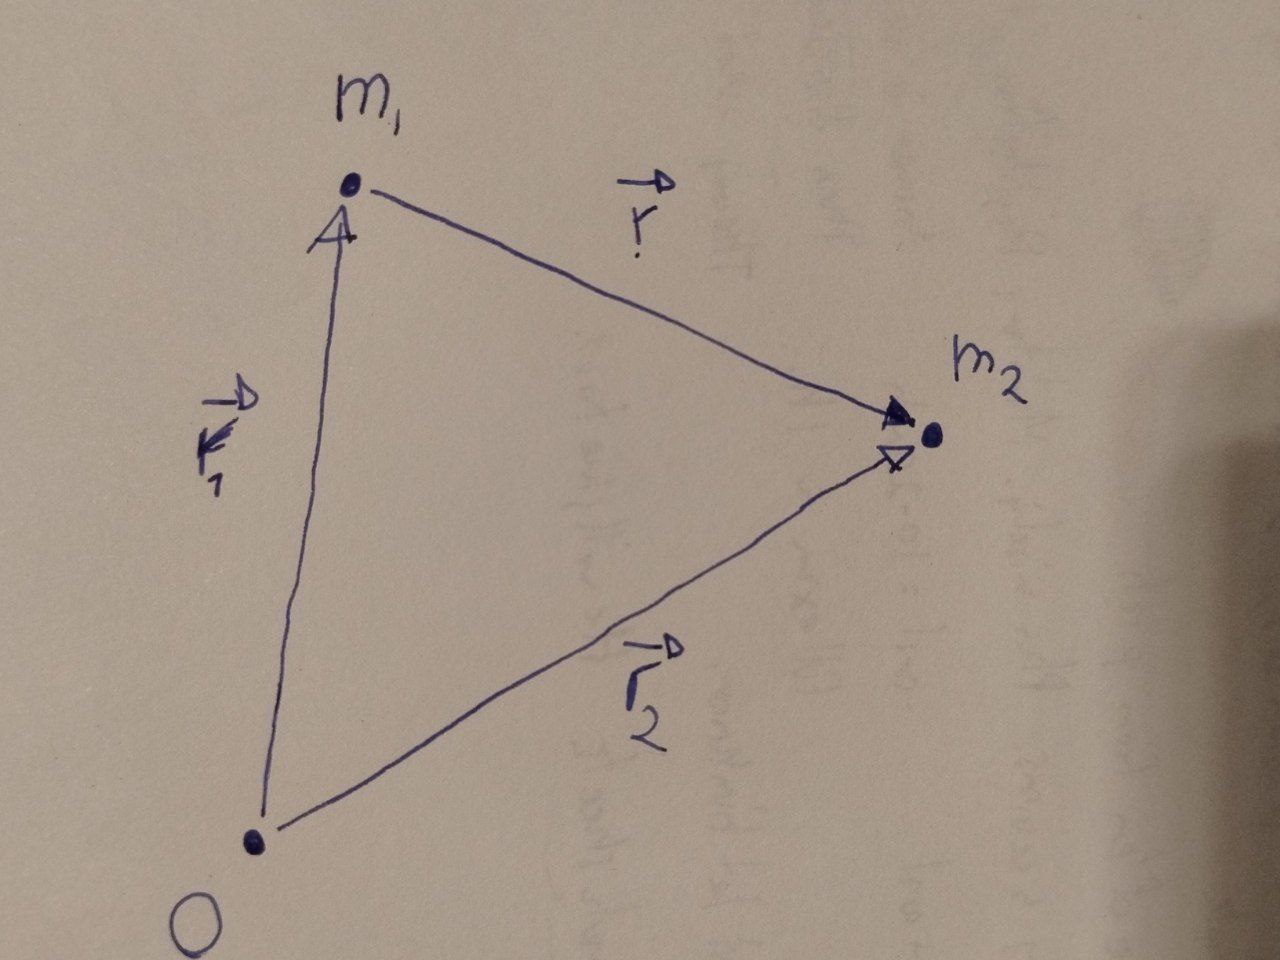
\includegraphics[width=\linewidth]{imm/ei_to_new.jpg} 
    %\caption{Gravitational \\  interaction of two masses}
    \vspace{12pt}
\end{minipage}
\end{figure}
\begin{minipage}[t]{0.48\textwidth}
    \vspace*{0pt} 
      We got two masses, $ m_{1}, m_{2} $, the origin, O, of the RF. \\ Each mass' position is identified by its own position vector.
	\begin{gather*}
\vec{r} = \vec{r}_{1}+\vec{r}_{2} \\
\vec{F}_{21}= - \frac{Gm_{1}m_{2}}{r^{2}} \hat{r} \\
\text{with } \hat{r} = \frac{\vec{r}}{|\vec{r}|}
	\end{gather*}
	   so, we see that m\textsubscript{2} is attracted. \\
	   P.S. $G = 6.67\times10^{-11} \frac{Nm^{2}}{kg^{2}} $
\end{minipage}

Introducing the second law of dynamics in the study, we have
\begin{gather*}
m_{2}\vec{a}_{2} = \vec{F}_{21} = - \frac{Gm_{1}m_{2}}{r^{2}} \hat{r} \\
\text{simplifying } m_{2} \text{ we obtain} \\
\vec{a}_{2} = - \frac{Gm_{1}}{r^{2}} \hat{r}  
\end{gather*}
We can express \textbf{a}\textsubscript{2} as 
\begin{gather*}
	\vec{a}_{2} = - \nabla \phi \text{ Gradient of the Gravitational Potential} \\
	\phi = - \frac{Gm_{1}}{r} \\
	\nabla^{2} \phi = -4\pi G \rho
\end{gather*}

We will use the Minkowski metric tensor 
\begin{equation}
	\eta_{\mu\nu} =
	\begin{pmatrix}
		-1 & 0 & 0 & 0 \\
		0 & +1 & 0 & 0 \\
		0 & 0 & +1 & 0 \\
		0 & 0 & 0 & +1 
	\end{pmatrix}
\end{equation}
 We will see also other symbols, like the Kristoffel one, or the Richie Tensor... \\
 But in the end the central goal is to derive the \emph{Einstein Equation}:
\begin{equation}
R_{\mu\nu} = \frac{1}{2} g_{\mu\nu}R = 8\pi G T_{\mu\nu}
\end{equation}

In GR particles move freely along \emph{straight lines} of a curved space-time. These are called \emph{geodesics}.

\paragraph{Example}
Two chalks, one on the desk, the other is launched in the air. Which one is accelerated?
From a GR perspective, the one in the air is moving along a geodesic, so it is the one moving freely, while the other is stopped from doing that by some interference/force. \\
In GR gravity is \emph{not} a force. 

\chapter{Math tools}
\section{A recap of SR}
\textbf{Lecture 2}
We will develop some of the necessary math on this framework. \\
Let's look at the Galilean Relativity. \\
Newtonian dynamics is based on three principles
\begin{enumerate}
	\item inertia
	\item $\vec{F} = m \vec{a}$
	\item action-reaction
\end{enumerate}
The first says something like \emph{An object at rest remains at rest, and an object in motion remains in motion at constant speed and in a straight line unless acted on by an unbalanced force}. \par
The second one says:
\[
	(2): \vec{F} = 0 \implies \vec{a} = 0 \implies (1)
\]

So, it seems the first principle is contained by the second, but we know that $\vec{F} = m \vec{a} $ is valid only in Inertial Frames (IF). \par
\paragraph{Galilean Relativity:} all the laws of \emph{mechanics} take the same form in every IF. (You can not distinguish two IF just by doing experiments.) \par
\begin{figure}
\begin{minipage}[t]{0.4\textwidth}
    \vspace*{0pt} 
    \centering
    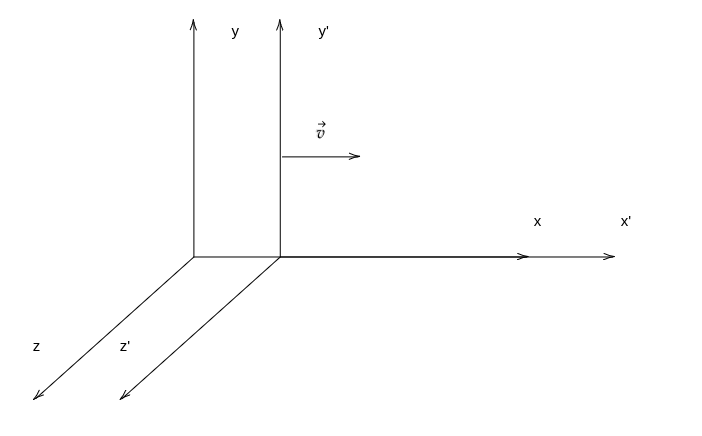
\includegraphics[width=\linewidth]{imm/galileianboost.png} 
    %\caption{G. Boost}
\end{minipage}

\end{figure}
\begin{minipage}[t]{0.4\textwidth}
    \vspace*{0pt}
    $
    \begin{cases}
    x' = x - vt \\
    y' = y \\
    z' = z \\
    t' = t
    \end{cases}$ \par
      $t = t' = 0 \implies O = O'$
\end{minipage} 
\bigskip

Taking the first derivative:
\begin{equation}
\begin{cases}
v_{x}' = v_{x} - v \\
v_{y}' = v_{y} \\
v_{z}' = v_{z} \\
\end{cases} \text{and for the second derivative: } \\
\begin{cases}
a_{x}' = a_{x} \\
a_{y}' = a_{y}\\
a_{z}' = a_{z}
\end{cases} \implies \vec{a}' = \vec{a}
\end{equation}
so also $\vec{F}' = \vec{F}$. And if \emph{m} is independent on the frame, we got
\begin{equation}
\vec{F}'=m \vec{a}' = \vec{F} = m \vec{a}
\end{equation}
\bigskip

Then there are Maxwell equations, people thanks to them find that EM-waves propagates with speed \emph{c} in the void. \par
But they found also that these equations were not invariant in Galilean Boosts. \par
Things started to go better when the idea of a preferred IF was ditched and Einstein decided to use Lorentz Transformations.\par

There are two postulates: \par
\begin{itemize}
	\item \emph{Relativity principle}: same as before but with \emph{physics} instead of \emph{mechanics}. \textbf{All the laws of physics ...}
	\item \emph{Speed of light}: in every IF, light propagates with constant speed, \emph{c}.
\end{itemize}
So we see that Galilean transformation become inconsistent with this, meanwhile stays valid for $\vec{v} \ll \vec{c}$.\par
As mentioned before, updated version of G. Boosts are Lorentz transformations (or Lorentz Boosts.)
\begin{equation}
\begin{cases}
	x' = \frac{x-vt}{\sqrt{1-(\frac{v}{c})^{2}}} \\
	y' = y \\
	z' = z \\
	t' = \frac{t- \frac{vx}{c^{2}}}{\sqrt{1-(\frac{v}{c})^{2}}}
\end{cases}
\end{equation}

To ensure the L.T. Is consistent we can perform three checks:
\begin{itemize}
	\item $v \ll c$
	\item v = 0
	\item dimensional check
\end{itemize}
People use a notation to make the L.T. easier to write: $\gamma(v) \equiv \frac{1}{\sqrt{1-(\frac{v}{c})^{2}}} $, so it becomes
\begin{equation}
\begin{cases}
x' = \gamma (x-vt) \\
y' = y \\
z' = z \\
t' = \gamma (t- \frac{vx}{c^{2}})
\end{cases}
\end{equation}

What happens to the transformation of velocity is: (v is fixed) 
\begin{equation}
\begin{cases}
dx' = \gamma(dx -vdt) \\
dy' = dy \\
dz' = dz \\
dt' = \gamma \left(dt - \frac{v dx}{c^{2}}\right)
\end{cases}
\end{equation}
 so 
\begin{equation}
\begin{cases}
 v_{x}' = \frac{dx'}{dt'} \\
 v_{y}' = \frac{dy'}{dt} = \frac{dy}{\gamma \left(dt - \frac{vdx}{c^{2}}\right)} = \frac{v_{y}}{\gamma \left(1- \frac{v v_{x}}{c^{2}}\right)} \\
v_{z}' = \frac{dz'}{dt} = ...
\end{cases}
\end{equation}
So we see that space-time changes also along other axes.\par

Now let's talk about space-time and its parts.

\paragraph{Space-time} space-time is a manifold. For now it is a collection of (t,x,y,z), four dimensional set of all the possible values of the coordinates.
\paragraph{Event} a point of space-time.
\paragraph{World line} path of a particle in space-time.

\begin{figure}
\centering
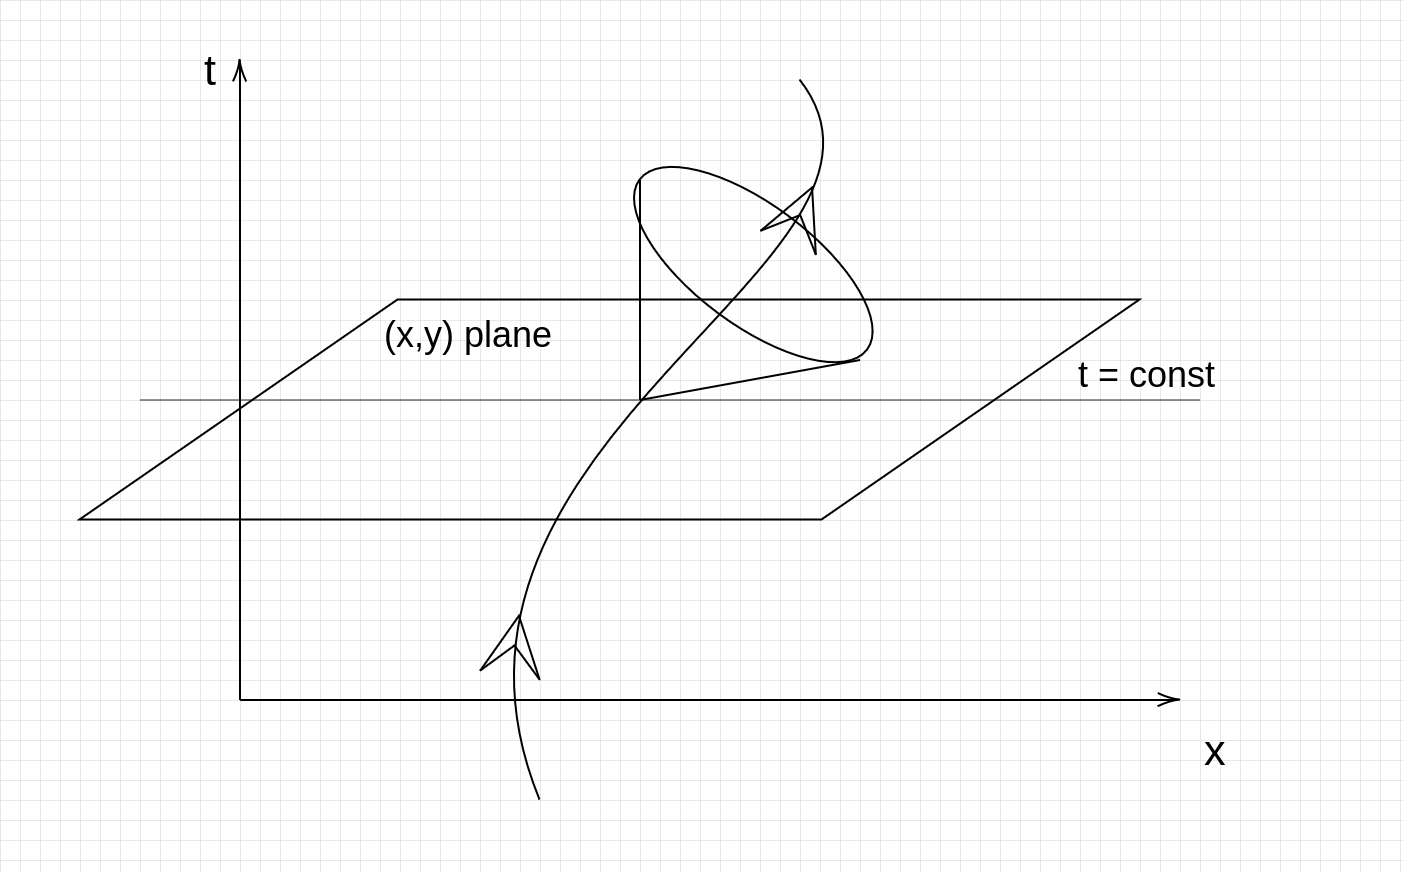
\includegraphics[width=\linewidth]{imm/WLLC.png}
\caption{LL of a particle which moves forward in time, we see also a light cone}
\label{mm:WLLC}
\end{figure}

There is no notion of absolute time anymore, because now it is dependent on the frame. 
Regarding the light-cone, after the event on the ( x,y ) plane, the particle can move \emph{only} inside the light-cone, in the appropriate direction (time forward).

Now let's talk about \textbf{Clock Synchronization.} \par
It is kinda easy if in in IF. In GR it is quite subtle instead. \par

\paragraph{Example:} Be me in Origin of a RF watching my clock (A). How to define \emph{t} at another generic location (B)??

\begin{figure}
\centering
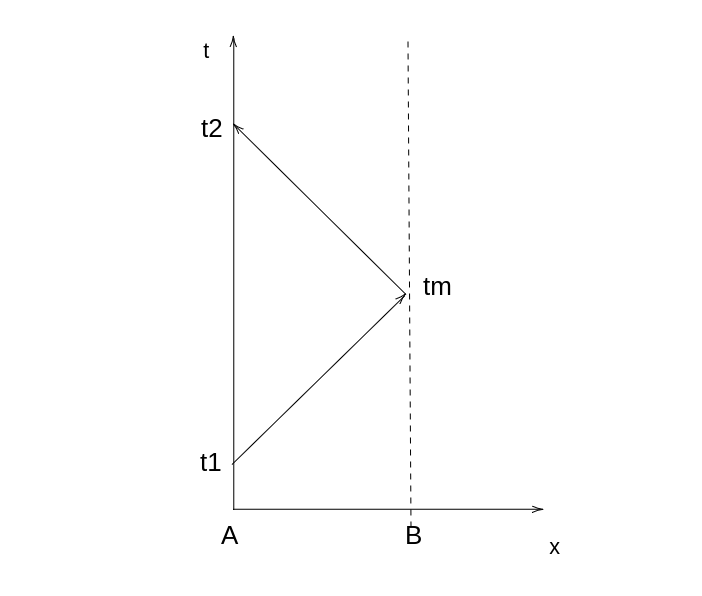
\includegraphics[width=\linewidth]{imm/segnale.png}
\caption{Reception and send of the signal}
\label{imm:segnale.png}
\end{figure}

I send a light ray at time \emph{t\textsubscript{1}} to B. I get the answer on \emph{t\textsubscript{2}}. There is symmetry between the two trajectories so \[
t_{m} = \frac{ t_{1} + t_{2} }{2}. 
\]
I say to my friend on B: "set your clock to t\textsubscript{m} when you receive the signal."
So, following this methodology, each point could have its own clock.

\paragraph{Proper time:} How to define proper time? \\
\emph{t} is the time coordinate. Let's introduce the metric tensor:
\begin{equation}
	\text{the Minkowski metric tensor: } \eta_{\mu \nu } = \begin{pmatrix}
	-1 & 0 & 0 & 0 \\
	0 & 1 & 0 & 0 \\
	0 & 0 & 1 & 0 \\
	0 & 0 & 0 & 1
	\end{pmatrix} 		
\end{equation}
for a Lorentz Transformation if I have 2 events E,F.
\begin{gather*}
	\text{Frame 1: } x_{F}^{\mu } = \left( t_{F}, x_{F}, y_{F}, z_{F} \right)\\
	x_{E} = \left( ... \right) \\
	\text{Frame 2: } x_{F}^{\mu' } = \left( t_{F'}, x_{F'}, y_{F'}, z_{F'} \right) \\
	x_{E}^{\mu' } = \left( ... \right)	 
\end{gather*}
same events in 2 different frames. \\
A Lorentz Transformation cornets these two events.

Be $\Delta s^{2}$ the Lorentz Invariant separation between E-F.
\begin{gather*}
\Delta s^{2} = -c \left( t_{F}-t_{E} \right)^{2} + \left( x_{F}- x_{E} \right)^{2} + \left( y_{F}-y_{E} \right)^{2} + \left( z_{F}-z_{E} \right)^{2} =\\
= -c (t_{F'}-t_{E'})^{2}  + (x_{F'}- x_{E'})^{2}  + (y_{F'}-y_{E'})^{2}  + (z_{F'}-z_{E'})^{2} \\
\Delta s^{2} = \eta_{\mu \nu } \Delta x^{\mu } \Delta x^{\nu } \\
\text{From this point we set } c = 1 \text{ just a rescaling} \\
\text{we have defined } \Delta x^{\mu } \equiv x_{F}^{\mu} - x_{F}^{\mu }, \text{with } \mu = 0,1,2,3.
\end{gather*}

So, repeating for clarity, the Lorentz Invariant separation is
\begin{equation}
\Delta s^{2} = \eta_{\mu  \nu } \Delta x^{\mu } x^{\nu } = \eta_{\mu'\nu'} \Delta x^{\mu '} \Delta x^{\nu'}
\end{equation}
Minkowski metric tensor does not change form if we change coordinates (Cartesian coordinates, meanwhile if we use like polar ones it changes for obvious reasons.) \par

if 
\begin{align*}
	\Delta s^{2} & > 0 \text{space-like separation} \\
		     &< \text{time-like, (it could be an actual LL for a massive particle)} \\
		     &= \text{light-like or null}
\end{align*}

Now we can define the \emph{proper time} as
\begin{equation}
	\Delta \tau^{2} \equiv - \Delta s^{2} \text{ or } \Delta \tau^{2} = - \eta_{\mu  \nu }\Delta x^{\mu } \Delta x^{\nu }
\end{equation}
So, if the proper time is \emph{positive} it is time-like.

If the segment \textbf{EF} marks the begin and end of the trajectory of a massive particle, $\Delta  \tau $, proper time, is the time elapsed on a clock sitting on a RF that moves with constant speed between E and F.
\\
Int the moving frame $\Delta \tau = \Delta t_{*}$ where \emph{t\textsubscript{*}} is the time coordinate of the moving frame. 
In a frame where I'm at rest this is how $\Delta t^{2}$ changes:
\begin{equation}
\Delta  \tau^{2} = + \Delta t^{2} - \Delta x^{2} - \Delta y^{2}- \Delta z^{2}.
\end{equation}

\section{Lecture 3}

The meaning of the Lorentz Invariant is that \textbf{events}, like $\left( E,F \right)$ exist before I define coordinates. It is a property of the two events.

So to recap what we did in the last lecture, be:
\begin{equation}
x_{E}^{\mu } \text{ and } x_{E}^{\mu'}
\end{equation}

\begin{figure}[ht]
\centering
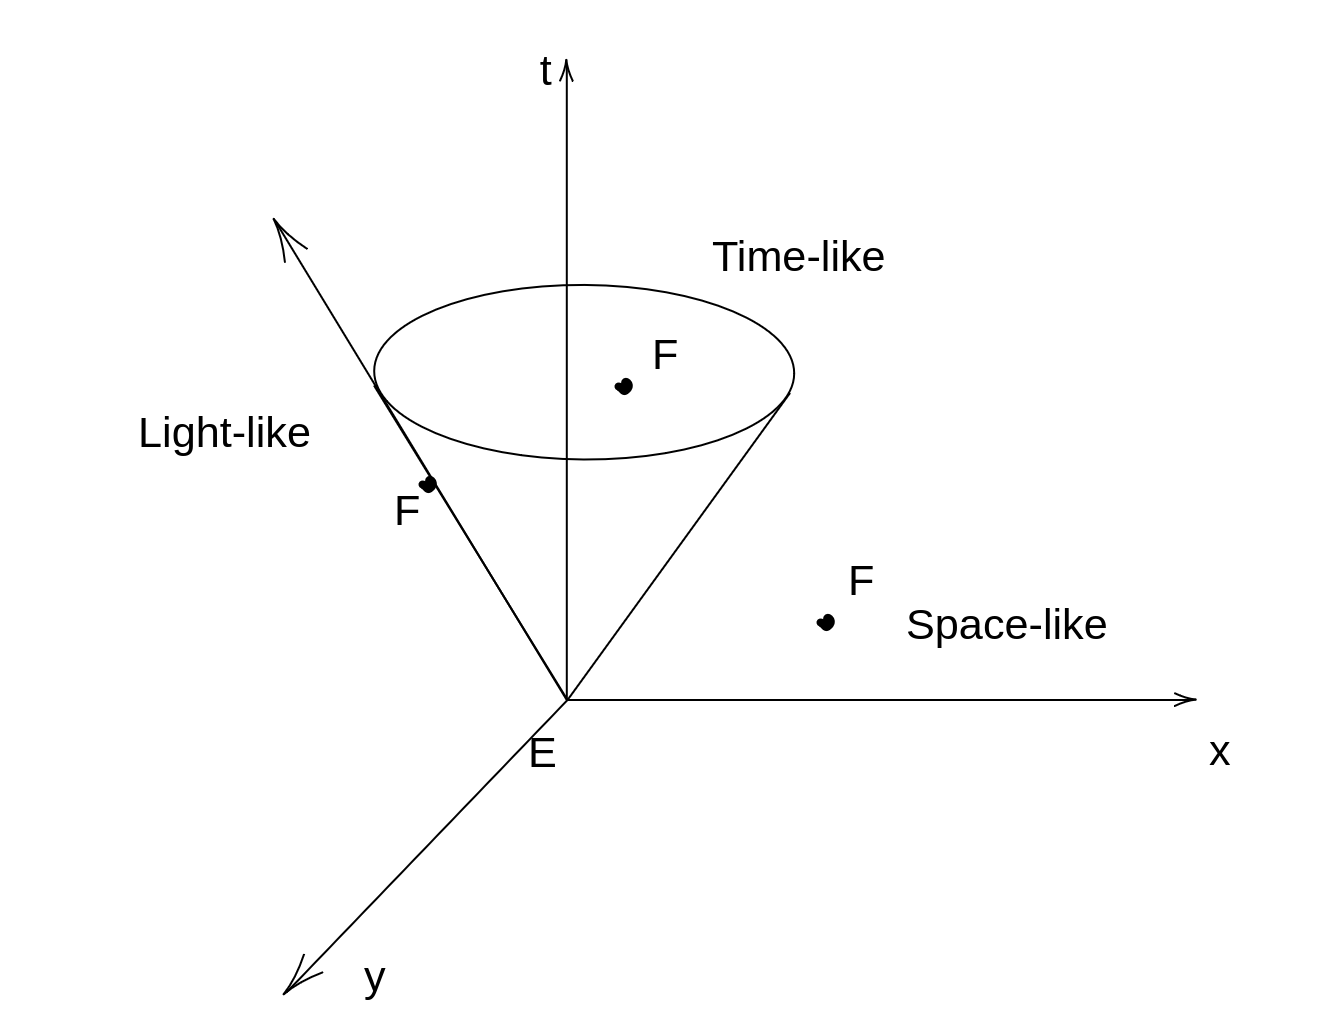
\includegraphics[width=\linewidth]{imm/lightcone.png}
\caption{Given event E, the separation \textbf{EF} could be of different types based on the position respect the light cone}
\label{imm:lightcone}
\end{figure}

If I have two events and computing $\Delta \tau $ gives a positive result, the separation is \textbf{time-like}.
This means that they could be on the WL of a massive particle moving at constant speed.

\paragraph{Physical meaning of $\Delta \tau $}
It's the time elapsed on a clock of the observer moving between E and F at constant speed.

This means that if I compute $\Delta \tau $ on the frame where the observer it is at rest, i get \[
\Delta \tau = \Delta t'
\]

Lets do an example:
\paragraph{Example}
\begin{figure}
\centering
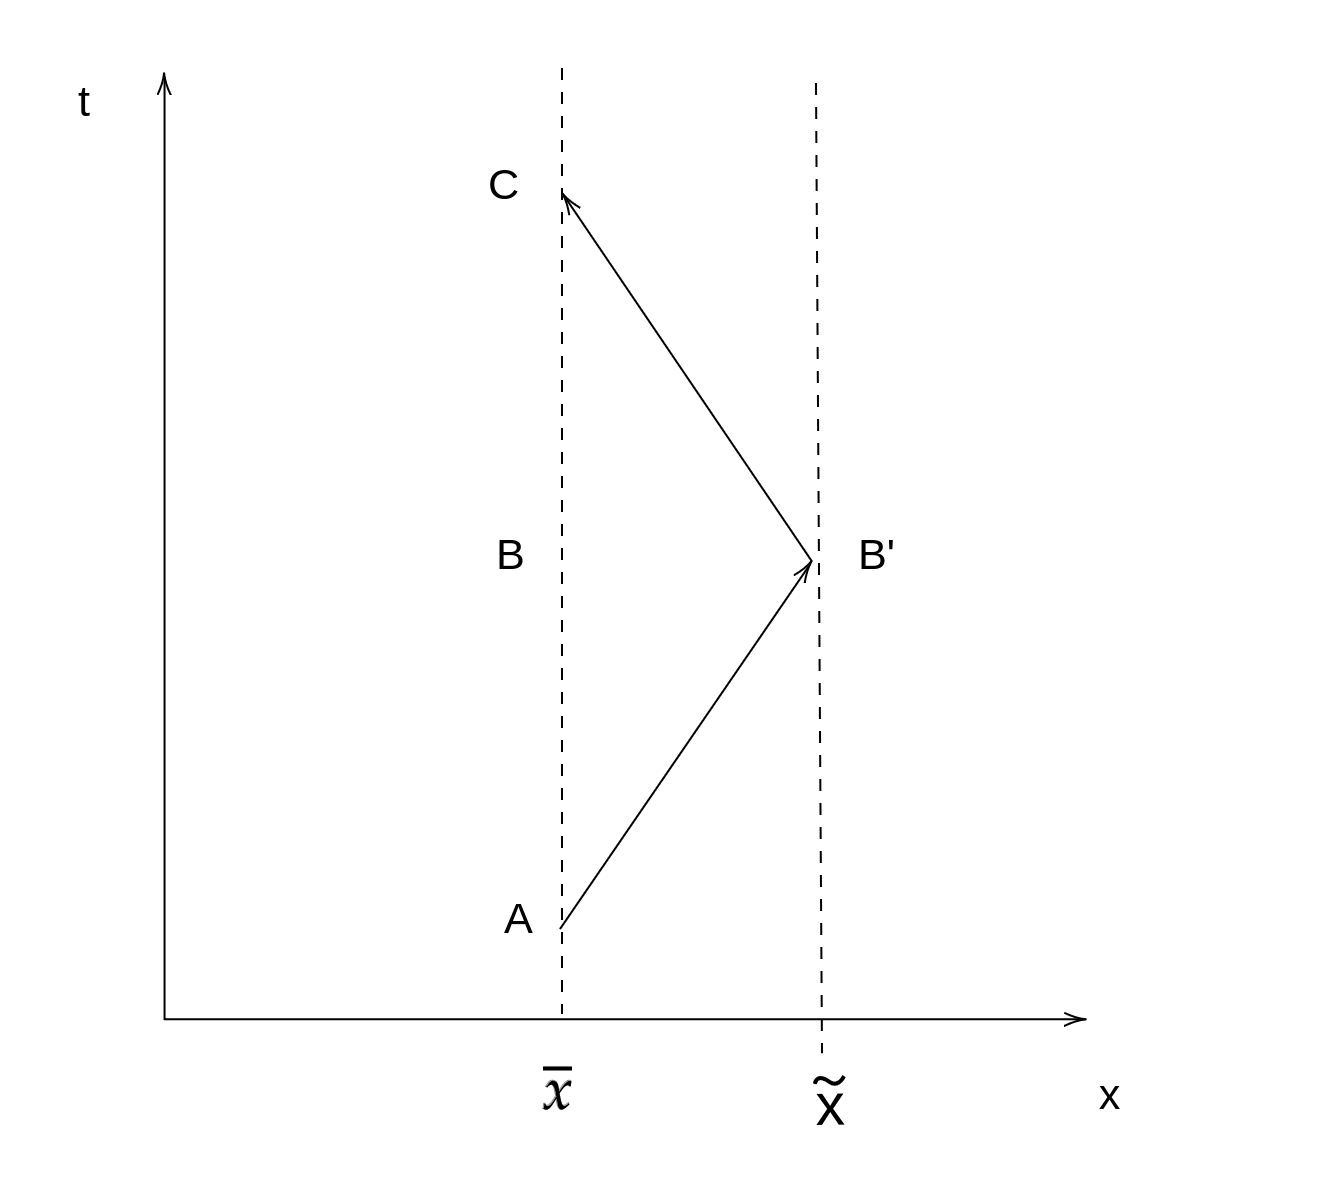
\includegraphics[width=\linewidth]{imm/examplelec3.png}
\caption{It is like the twin paradox.}
\label{imm:examplelec3}
\end{figure}

In fig. \ref{imm:examplelec3} we see the straight line \textbf{ABC} that is the WL of a object not moving. 
Computing its proper time will be:
\begin{equation}
\Delta \tau_{ABC} = \left( t_{c}-t_{A} \right)
\end{equation}
But for the other WL, of a object moving at constant speed between \textbf{AB'} and \textbf{B'C}, first thing first, we see that
\begin{gather*}
t_{B} = t_{B'} \\
\text{ and so } \\
\Delta \tau_{AB'C} = 2 \sqrt{\left( t_{B} - t_{A} \right)^{2} - \left( \tilde{x} - \bar{x} \right)^{2}} = \Delta \tau_{ABC} \sqrt{1 - \left( \frac{v}{c}  \right)^{2}} \\
\implies \Delta \tau_{AB'C} < \Delta \tau_{ABC}
\end{gather*}

This means that I have the longest \textbf{proper time} when I don't move.

We can do one more generalization: by parametrize the WL with a quantity $\lambda $ we get
\begin{gather*}
x^{\mu }\left( \lambda  \right) \\
\Delta \tau = \int \sqrt{- \eta_{\mu \nu } \frac{dx^{\mu }}{d\lambda } \frac{dx^{\nu }}{d\lambda }} d\lambda \text{ that is a time like trajectory. }
\end{gather*}

Enough with proper time.

\subsection{Tensor Calculus}
Be a Lorentz Group, we want to look for the transformations.
\begin{equation}
x^{\mu } \to x^{\mu'} = \Lambda^{\mu'}_{\mu } x^{\mu }
\end{equation}
we see that it is a linear transformation. An example to see better what are we doing could be
\begin{equation}
x^{0'} = \Lambda^{0'}_{0}x^{0} + \Lambda^{0'}_{1}x^{1} + \Lambda^{0'}_{2}x^{2} + \Lambda^{0'}_{3}x^{3}
\end{equation}
What we need to know is that $\Lambda^{\mu'}_{\mu }$ is a constant matrix.

We see that $\Lambda $   is a constant matrix.

We want to find linear transformations such that 
\begin{equation}
\Delta s^{2} = \eta_{\mu \nu } \Delta x^{\mu }\Delta x^{\nu } = \eta_{\mu' \nu'} \Delta x^{\mu'}\Delta x^{\nu'}
\end{equation}
So the Lorentz Invariant is still invariant. (WTF)

Now, because a SR property: if I move from IF to another, $\eta$ is still unchanged. So \[
\eta_{\mu \nu } = \eta_{\mu' \nu'}
\]

We have to say that Minkowski assumes cartesian coordinates.

The question now is: What trivial transformations leave $\Delta s^{2}$ unchanged?

\paragraph{Translations}
\begin{gather*}
\eta_{\mu  \nu }\Delta x^{\mu }x^{\nu } = \eta_{\mu' \nu'}\left( \Lambda^{\mu'}_{\mu }\Delta x^{\mu } \right) \left( \Lambda^{\nu'}_{\nu }\Delta x^{\nu } \right) \\
\implies \eta_{\mu  \nu } = \eta_{\mu' \nu'} \Lambda^{\mu'}_{\mu }\Lambda^{\nu'}_{\nu } \\
\text{ this obviously needs to be valid } \forall \Delta x^{\mu } \\
\text{ an alternative notation could be } \eta = \Lambda^{T} \eta \Lambda \\
\end{gather*}
We will use just the first notation, because we need to get good at tensors.

To be more concrete:
\begin{equation}
\Lambda^{\mu'}_{\mu } = \begin{pmatrix}
\Lambda^{0'}_{0} & \Lambda^{0'}_{1} & \Lambda^{0'}_{2} & \Lambda^{0'}_{3} \\
\Lambda^{1'}_{0} & ... & ... & ... \\
\Lambda^{2'}_{0} & ... & ... & ... \\
\Lambda^{3'}_{0} & ... & ... & ...
\end{pmatrix} 
\end{equation}

\paragraph{Rotations} 


Rotations are a kind of transformation of the type:
\begin{gather*}
x_{i'} = R_{i i'} x_{i} \\
\text{ or } R^{T} \mathbb{I} R = \mathbb{I} \\
\text{ with } RR^{T} = R^{T}R = \mathbb{I}
\end{gather*}

it could be something like
\begin{equation} \Lambda^{\mu'}_{\mu } = 
\begin{pmatrix}
cosh \eta  & -sinh \eta   & 0 & 0 \\
-sinh \eta  & cosh \eta  & 0 & 0 \\
0 & 0 & 1 & 0 \\
0 & 0 & 0 & 1
\end{pmatrix} 
\end{equation}
this one is a boost along the $x$ direction. If we do some computing we find that 
\[
tanh \eta \equiv v
\]
so this is the same of the L.T. we saw last week. \par

Rotations do not change the time coordinate. The point was to tell what L.T. is in this language.

\paragraph{Vectors}


I have a generic vector, \textbf{do i need to  specify about the RF} where it is defined, so in a specific spacetime location? {\tiny yes} \par

In newtonian mechanics parallel vectors are the same because I can superpose them, I can move them around, also to use the parallelogram rule to get a sum. \par
$\implies$If I have 3D euclidean space there is no ambiguities about where i move my vectors.\par
\textbf{BUT} in a sphere:

\noindent
\begin{minipage}[t]{0.45\textwidth}
	\vspace*{0pt}
\tikzset{every picture/.style={line width=0.4pt}} %set default line width to 0.75pt        

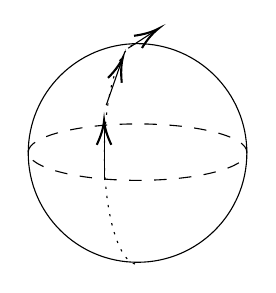
\begin{tikzpicture}[x=0.4pt,y=0.4pt,yscale=-1,xscale=1]
%uncomment if require: \path (0,300); %set diagram left start at 0, and has height of 300

%Shape: Circle [id:dp6654577831806846] 
\draw   (205.5,152.75) .. controls (205.5,98.21) and (249.71,54) .. (304.25,54) .. controls (358.79,54) and (403,98.21) .. (403,152.75) .. controls (403,207.29) and (358.79,251.5) .. (304.25,251.5) .. controls (249.71,251.5) and (205.5,207.29) .. (205.5,152.75) -- cycle ;
%Shape: Ellipse [id:dp25748828027722603] 
\draw  [dash pattern={on 4.5pt off 4.5pt}] (205.5,152) .. controls (205.5,137.92) and (249.71,126.5) .. (304.25,126.5) .. controls (358.79,126.5) and (403,137.92) .. (403,152) .. controls (403,166.08) and (358.79,177.5) .. (304.25,177.5) .. controls (249.71,177.5) and (205.5,166.08) .. (205.5,152) -- cycle ;
%Shape: Arc [id:dp3672101138168469] 
\draw  [draw opacity=0][dash pattern={on 0.84pt off 2.51pt}] (301.86,253.06) .. controls (286.41,249.01) and (274.25,206.07) .. (274.25,153.69) .. controls (274.25,100.16) and (286.95,56.49) .. (302.88,54.1) -- (304.25,153.69) -- cycle ; \draw  [dash pattern={on 0.84pt off 2.51pt}] (301.86,253.06) .. controls (286.41,249.01) and (274.25,206.07) .. (274.25,153.69) .. controls (274.25,100.16) and (286.95,56.49) .. (302.88,54.1) ;  
%Straight Lines [id:da2694092326525188] 
\draw    (274,177.5) -- (274,125.5) ;
\draw [shift={(274,123.5)}, rotate = 90] [color={rgb, 255:red, 0; green, 0; blue, 0 }  ][line width=0.75]    (21.86,-6.58) .. controls (13.9,-2.79) and (6.61,-0.6) .. (0,0) .. controls (6.61,0.6) and (13.9,2.79) .. (21.86,6.58)   ;
%Straight Lines [id:da8503547294122475] 
\draw    (276,109.5) -- (290.34,68.39) ;
\draw [shift={(291,66.5)}, rotate = 109.23] [color={rgb, 255:red, 0; green, 0; blue, 0 }  ][line width=0.75]    (21.86,-6.58) .. controls (13.9,-2.79) and (6.61,-0.6) .. (0,0) .. controls (6.61,0.6) and (13.9,2.79) .. (21.86,6.58)   ;
%Straight Lines [id:da6949662065564377] 
\draw    (295.88,58.1) -- (321.32,41.59) ;
\draw [shift={(323,40.5)}, rotate = 147.02] [color={rgb, 255:red, 0; green, 0; blue, 0 }  ][line width=0.75]    (21.86,-6.58) .. controls (13.9,-2.79) and (6.61,-0.6) .. (0,0) .. controls (6.61,0.6) and (13.9,2.79) .. (21.86,6.58)   ;

\end{tikzpicture}
\end{minipage}
\begin{minipage}[t]{0.48\textwidth}
    \vspace*{0pt} 
    I have this vector at the equator tangent to the surface. If I transport it to the pole i get a different vector.		
\end{minipage}
\bigskip

There are ambiguities. So in a non-flat space we need a \textbf{different} procedure. \par
A vector field is a map between:
\[
x^{\mu } \to v^{\mu }
\]
where $x^{\mu }$ is an event and $v^{\mu }$ is a vector. \par

Let's define: \textbf{Tangent space T\textsubscript{P}}.\par
Given an event $P$ we define the tangent space $T_{P}$ as all the vectors in $P$.\par

Instead of having spacetime we have a sphere.

\noindent
\begin{minipage}[t]{0.48\textwidth}
    \vspace*{0pt}
    

\tikzset{every picture/.style={line width=0.75pt}} %set default line width to 0.75pt        

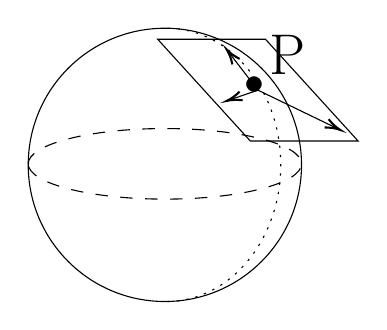
\begin{tikzpicture}[x=0.5pt,y=0.5pt,yscale=-1,xscale=1]
%uncomment if require: \path (0,300); %set diagram left start at 0, and has height of 300

%Shape: Circle [id:dp6654577831806846] 
\draw   (17.5,138.75) .. controls (17.5,84.21) and (61.71,40) .. (116.25,40) .. controls (170.79,40) and (215,84.21) .. (215,138.75) .. controls (215,193.29) and (170.79,237.5) .. (116.25,237.5) .. controls (61.71,237.5) and (17.5,193.29) .. (17.5,138.75) -- cycle ;
%Shape: Ellipse [id:dp25748828027722603] 
\draw  [dash pattern={on 4.5pt off 4.5pt}] (17.5,138) .. controls (17.5,123.92) and (61.71,112.5) .. (116.25,112.5) .. controls (170.79,112.5) and (215,123.92) .. (215,138) .. controls (215,152.08) and (170.79,163.5) .. (116.25,163.5) .. controls (61.71,163.5) and (17.5,152.08) .. (17.5,138) -- cycle ;
%Shape: Arc [id:dp3672101138168469] 
\draw  [draw opacity=0][dash pattern={on 0.84pt off 2.51pt}] (118.33,237.5) .. controls (163.51,236.96) and (200,192.96) .. (200,138.75) .. controls (200,84.76) and (163.8,40.88) .. (118.86,40.01) -- (117.5,138.75) -- cycle ; \draw  [dash pattern={on 0.84pt off 2.51pt}] (118.33,237.5) .. controls (163.51,236.96) and (200,192.96) .. (200,138.75) .. controls (200,84.76) and (163.8,40.88) .. (118.86,40.01) ;  
%Shape: Parallelogram [id:dp887464464445318] 
\draw   (111.1,48) -- (189,48) -- (255.9,121.5) -- (178,121.5) -- cycle ;
%Straight Lines [id:da3128101776711285] 
\draw    (183.5,84.75) -- (241.2,112.63) ;
\draw [shift={(243,113.5)}, rotate = 205.79] [color={rgb, 255:red, 0; green, 0; blue, 0 }  ][line width=0.75]    (10.93,-3.29) .. controls (6.95,-1.4) and (3.31,-0.3) .. (0,0) .. controls (3.31,0.3) and (6.95,1.4) .. (10.93,3.29)   ;
%Straight Lines [id:da05720579900710121] 
\draw    (183.5,84.75) -- (162.22,57.09) ;
\draw [shift={(161,55.5)}, rotate = 52.43] [color={rgb, 255:red, 0; green, 0; blue, 0 }  ][line width=0.75]    (10.93,-3.29) .. controls (6.95,-1.4) and (3.31,-0.3) .. (0,0) .. controls (3.31,0.3) and (6.95,1.4) .. (10.93,3.29)   ;
%Straight Lines [id:da5083189086137138] 
\draw    (183.5,84.75) -- (162.89,91.85) ;
\draw [shift={(161,92.5)}, rotate = 340.99] [color={rgb, 255:red, 0; green, 0; blue, 0 }  ][line width=0.75]    (10.93,-3.29) .. controls (6.95,-1.4) and (3.31,-0.3) .. (0,0) .. controls (3.31,0.3) and (6.95,1.4) .. (10.93,3.29)   ;

% Text Node
\draw (172,73.4) node [anchor=north west][inner sep=0.75pt]  [font=\Large]  {$\bullet $};
% Text Node
\draw (190,43) node [anchor=north west][inner sep=0.75pt]   [align=left] {{\huge P}};


\end{tikzpicture}

\end{minipage}
\begin{minipage}[t]{0.48\textwidth}
    \vspace*{0pt} 
	Define a plane tangent to the sphere only in $P$. All vectors that lie there $\in T_{P}$.    
\end{minipage}
\bigskip


$T_{P}$ is a \textbf{vector space}:
\[
	V,W \in T_{P} \implies \alpha V + \beta W, \left( \alpha , \beta \in \mathbb{R} \right) \in T_{P}
\]
So if there is a vector there is also the inverse vector.\par
Whenever i have a vector space, I can define infinite basis independently on the coordinate choice. The nUmber of elements in the basis is equal to the dimension of the space, in our case 4 elements.\par
Obviously if I define the basis its elements need to be Linearly Independent. 

\paragraph{Basis}
Given a generic vector $V \in T_{P}$, I can define $V$ regardless the coordinate system I'm using. So we can say \emph{meTaphorically} that $V$ exists before I define coordinates.\par

Be our basis:
\[
\hat{e}_{\left( \mu  \right)}, \text{ with } \mu = 0,1,2,3	
\]
those indices are label, does not mean "tensor". So my basis is made of \[
\hat{e}_{\left( 0 \right)}, \hat{e}_{\left( 1 \right)}, \hat{e}_{\left( 2 \right)}, \hat{e}_{\left( 3 \right)}
\]
Now we can talk about
\paragraph{Components}
given a generic vector $v$ 
\[
V = V^{0}\hat{e}_{\left( 0 \right)} + V^{1}\hat{e}_{\left( 1 \right)} + V^{2}\hat{e}_{\left( 2 \right)} + V^{3}\hat{e}_{\left( 3 \right)} =  V^{\mu }\hat{e}_{\left( \mu  \right) }
\]
using repeating indices we get the last equivalence.

$V^{\mu }$ are components of the vector $V$ in this specific frame. \par
In another frame $V^{\mu '}$ could not be the same:
\[
	V = V^{\mu }\hat{e}_{\left( \mu  \right)} = V^{\mu '}\hat{e}_{\left( \mu ' \right)}
\]

\textbf{Question:} how do components transform?
\paragraph{covariant vector}: is a math object whose components transform based on position
\[
V^{\mu '} = \Lambda^{\mu '}_{\mu }V^{\mu }
\]
These are not the only covariant vectors (?).

If you have a generic WL or path, you can parametrize the position by a $\lambda$ in this way:
\[
x^{\mu }\left( \lambda  \right)
\]
And taking its first derivative you get something similar to the four-velocity
\[
u^{\mu }\sim \frac{dx^{\mu }}{d\lambda }
\]
(I say similar because four-velocity is defined like $u^{\mu } = \frac{dx^{\mu }}{d\tau }$).

If I do a L.T. $x^{\mu }$ will change but $\lambda $ won't.
\[
u^{\mu '} = \Lambda^{\mu '}_{\mu }u^{\mu }
\]
I can get a more general definition of what a vector is by following this procedure:
choose basis $\to$ find components $\to$ study how components change if i change position or basis.

\paragraph{Second definition}: Transformation of the basis vectors. The question is "how to relate $\hat{e}_{\left( \mu  \right)}$ to $\hat{e}_{\left( \mu ' \right)}$?"

We will take advantage of \textbf{invariance}. 
\[
V = V^{\mu }\hat{e}_{\left( \mu  \right) } = V^{\mu '}\hat{e}_{\left( \mu ' \right)} = \left( \Lambda^{\mu '}_{\mu }V^{\mu } \right)\hat{e}_{\left( \mu ' \right)}
\]
That's possible \textbf{only} if $\hat{e}_{\left( \mu  \right)} = \Lambda^{\mu '}_{\mu }\hat{e}_{\left( \mu ' \right)}$.

An inverse of LT it is also a LT, so
\begin{gather*}
\Lambda^{\mu '}_{\mu }\Lambda^{\mu }_{\nu '} = \delta^{\mu '}_{\nu '} \\
\Lambda^{\mu }_{\mu '}\Lambda^{\mu '}_{\nu } = \delta^{\mu }_{\nu }	
\end{gather*}
Those are Kroneker's delta and they are an Identity matrix.

Now we can study how basis vectors change.
\begin{gather*}
\hat{e}_{\left( \mu  \right)} = \Lambda^{\mu '}_{\mu }\hat{e}_{\left( \mu ' \right)} \\
\Lambda^{\mu }_{\nu '}\hat{e}_{\left( \mu  \right)} = \Lambda^{\mu '}_{\mu }\Lambda^{\mu }_{\nu '} \hat{e}_{\mu '} \\
\Lambda^{\mu }_{\nu '}\hat{e}_{\left( \mu  \right)} = \delta^{\mu '}_{\nu '}\hat{e}_{\left( \mu ' \right)} \\
\Lambda^{\mu }_{\nu '}\hat{e}_{\left( \mu  \right)} = \hat{e}_{\left( \nu ' \right)} \\ 
\text{ so } \hat{e}_{\left( \nu ' \right)} = \Lambda^{\mu }_{\nu '}\hat{e}_{\left( \mu  \right)}
\end{gather*}
	
\section{Lecture 4}

\subsubsection{Brief recap of lec3}
We defined vectors
\begin{itemize}
	\item localized at each spacetime point
	\item for each event P we defined the tangent space $T_{P}$
	\item there is linear combination inside $T_{P}$
	\item it has a basis
	\item Vectors and basis transform under LT Group.
\end{itemize}

\subsubsection{Dual vectors}
Using old terminology they are covariant, so with lower indices. Meanwhile contravariant do have upper indices.

Let's start with defining the \textbf{dual space} of a vector space:
\emph{Given a vector space (for concreteness T\textsubscript{P})}, we define the \textbf{dual space} $T_{P}^{*}$ as the space of linear maps between $T_{P}$ and $\mathbb{R}$.

\paragraph{Example}
Being $\omega  \in T_{P}^{*}$, $V \in T_{P}$ then
\[
	\omega \left( V \right) \in \mathbb{R}
\]
Linearity tells me that 
\[
\omega \left( \alpha V + \beta  W \right) = \alpha \omega \left( V \right) + \beta \omega \left( W \right)
\]

\paragraph{1\textsuperscript{st} statement}: The dual space is a vector space.
\[
	\left( \alpha \omega  + \beta \eta  \right)\left( v \right) = \alpha \omega \left( v \right) + \beta \eta \left( v \right)
\]
\paragraph{2\textsuperscript{nd} statement}: What is the dual of the dual?
\[
	\left( T_{P}^{*} \right)^{*} = T_{P} \implies v\left( \omega  \right) = \omega \left( v \right) \in \mathbb{R}
\]

\paragraph{Basis for T\textsubscript{P}\textsuperscript{*}}: $\hat{o}^{\left( \mu  \right)}$. \\
How to define this? Definition is
\[
\hat{o}^{\left( \mu  \right)}\left( \hat{e}_{\left( \nu  \right)} \right) \equiv \delta^{\mu }_{\nu }
\]
Now let's see if we can get how dual vectors work with vectors.
If I have:
\begin{itemize}
	\item generic item of $T_{P}$: $V = V^{\nu }\hat{e}_{\left( \nu  \right)}$
	\item generic item of $T_{P}^{*}: \omega = \omega_{\mu }\hat{o^{\left( \mu  \right)}}$ 
\end{itemize} 

I can compute:
\begin{gather*}
\omega \left( v \right) = \omega_{\mu }\hat{o}^{\left( \mu  \right)}\left( v^{\nu }\hat{e}_{\left( \nu  \right)} \right) =  \\
= \omega_{\mu }v^{\nu }\hat{o}^{\left( \mu  \right)}\left( \hat{e}_{\left( \nu  \right)} \right) = \omega_{\mu } v^{\nu } \delta^{\mu}_{\nu } = \omega_{\mu }v^{\mu }
\end{gather*}

\noindent\fbox{\begin{minipage}{\textwidth}
Once we know this we can do an \textbf{exercise}: show the way $\omega_{\mu '}$ transform.
What to do is to start from $\Lambda $ equality.\\
\end{minipage}} \\

What is the example of a dual vector? \\
\[
A_{\mu '} = \Lambda_{\mu }^{\mu '} A_{\mu }
\]
the gradient is a beautiful example of a \emph{dual vector}.
\[
A_{\mu } = \frac{\partial\phi }{\partial x^{\mu }} \text{  ;   } A_{\mu '} = \frac{\partial\phi }{\partial x^{\mu '}}
\]
This is useful to define LTs, in this way
\[
\frac{\partial\phi }{\partial x^{\mu '}} = \frac{\partial\phi }{\partial x^{\mu }} \frac{\partial x^{\mu }}{\partial x^{\mu '}} \to A_{\mu '} = \frac{\partial x^{\mu }}{\partial x^{\mu '}}A_{\mu }
\]
the LT is the last partial derivative. \\

There is a \emph{more compact} notation tho write partial derivatives that is
\[
\partial_{\mu } \phi \equiv \frac{\partial\phi }{\partial x^{\mu }}
\]

\subsection{Tensors}

Tensors are generalization of dual vectors and vectors. \\
They are \emph{multilinear maps}, i.e. functions of several variables and linear for all of them. For each tensor of \emph{rank} (k,l), we have
\[
T_{P}^{*}\times \ldots \times T_{P}^{*} \times T_{P}\times \ldots \times T_{P} \to \mathbb{R} \]
Where each dual vector space is present \textbf{k}-times, and vector space \textbf{l}-times.

Now let's see what is multilinearity on the combat field.

\noindent\fbox{
	\begin{minipage}{0.95\textwidth}
	Be a (1,1) tensor:
	\begin{itemize}
		\item $\alpha , \beta , \gamma , \delta \in \mathbb{R}$
		\item $\omega , \eta  \in T_{P}^{*}$
		\item v,w $\in $ T\textsubscript{P}
	\end{itemize}
	Given these we have
	\begin{equation}
	T\left( \alpha \omega + \beta \eta , \gamma v + \delta w \right) = \\
	= \alpha \gamma T\left( \omega , v \right) + \beta \delta T\left( \eta , w \right) + \alpha \delta T\left( \omega , w \right) + \beta \gamma T\left( \eta ,v \right)
	\end{equation}

\end{minipage}}

Once we have this general definition, let's take one step back:
\begin{itemize}
	\item Scalar $\to$ (0,0) tensor
	\item Vector $\to$ (1,0) tensor
	\item Dual vector $\to$ (0,1) tensor
\end{itemize}

\subsubsection{Tensor product}
Be:
\begin{itemize}
	\item T, rank (k,l) tensor
	\item S, rank (m,n) tensor
\end{itemize} 
We want to understand the action of $\otimes$. \\
So we know that $T\otimes S$ outputs (k+m, l+n) tensor. In particular,
\begin{gather*}
	T\otimes S \left[\omega^{\left( 1 \right)}, \ldots, \omega^{\left( k \right)}, \omega^{\left( k+1 \right)}, \ldots , \omega^{\left( k+m \right)}, v^{\left( 1 \right)}, \ldots , v^{\left( l \right)}, v^{\left( l+1 \right)}, \ldots , v^{\left( l+n \right)}\right] \equiv \\
	\equiv T\left( \omega^{\left( 1 \right)}, \ldots , \omega^{\left( k \right)}, v^{\left( 1 \right)}, \ldots , v^{\left( l \right)} \right) \times S\left( \omega^{\left( k+1 \right)}, \ldots , \omega^{\left( k+m \right)}, v^{\left( l+1 \right)}, \ldots , v^{\left( l+n \right)} \right) \\
	\implies T \otimes S \neq S \otimes T
\end{gather*}
so tensors do not commute.\\

\subsubsection{Basis for a tensor}
Let \emph{T} be a generic tensor with rank (k,l), \emph{basis} is given by
\[
\hat{e}_{\left( \mu_{1} \right)} \otimes \ldots \otimes \hat{e}_{( \mu_{k})} \otimes  \hat{o}^{\left( \nu_{1} \right)} \otimes \ldots \otimes \hat{o}^{(\nu_{l})}
\]

 A tensor can be written as 
 \[
 T = T^{\mu_{1}, \ldots , \mu_{k}}_{\nu_{1}, ..., \nu_{l}} \left( \hat{e}_{\left( \mu_{1} \right)} \otimes \ldots  \right) = T^{\mu_{1}^{'}, \ldots , \mu_{k}^{'}}_{\nu_{1}^{'}, \ldots , \nu _{l}^{'}}\left( \hat{e}_{\left( \mu_{1}^{'}  \right)} \otimes \ldots  \right)
 \]
So the tensor is always the same, the thing that changes is its components, because a change of RF I think.

We will often write the components instead of the actual tensor, but it is our convention to think they are equivalent.

This is how the components are related:
\begin{gather*}
\hat{e}_{\left( \mu ' \right)} = \Lambda^{\mu }_{\mu '} \hat{e}_{\left( \mu  \right)} \\
\hat{o}^{\left( \mu ' \right)} = \Lambda^{\mu '}_{\mu }\hat{o}^{\left( \mu  \right)} \\
\implies T = T^{\mu_{1}, \ldots , \mu_{k}}_{\nu_{1}, \ldots , \nu_{l}} \left( \Lambda^{\mu_{1}'}_{\mu_{1}} \hat{e}_{\left( \mu_{1}' \right)} \otimes \ldots  \right)
\end{gather*}
So we find, as result, that when I change frame
\begin{equation}
T^{\mu_{1}', \ldots , \mu_{k}'}_{\nu_{1}', \ldots , \nu_{k}'} = \Lambda^{\mu_{1}'}_{\mu_{1}} \ldots \Lambda^{\nu_{1}}_{\nu_{1}'} \ldots T^{\mu_{1}, ..., \mu_{k}}_{\nu_{1}, \ldots , \nu_{l}}
\end{equation}


\section{Lec 5}
\subsection{Transformations}
The goal is to find what is this $T^{\mu_{1}', \ldots , \mu_{k}'}_{\nu_{1}', \ldots , \nu_{l}'}= ?$.
\begin{equation}
T = T^{\mu_{1}, \ldots , \mu_{k}}_{\nu_{1, \ldots , \nu_{l}}} \left( \hat{e}_{\left( \mu_{1} \right)} \otimes \ldots  \right) = T^{\mu_{1}', \ldots , \mu_{k}'}_{\nu_{1}', \ldots , \nu_{l}'} \left( \hat{e}_{\left( \mu_{1}' \right)} \otimes \ldots  \right)
\end{equation}
I know two facts:
\begin{equation}
\begin{cases}
\hat{e}_{\mu '} = \Lambda^{\mu }_{\mu '} \hat{e}_{\left( \mu  \right)} \\
\hat{o}^{\mu '} = \Lambda^{\mu' }_{\mu } \hat{o}^{\mu } \\
\end{cases}
\end{equation}
and also the \emph{inverse.} \par

So i apply the Lambda transformation to each term of the basis and I get the following
\begin{equation}
T^{\mu_{1}', \ldots , \mu_{k}'}_{\nu_{1}', \ldots , \nu_{l}' } = \left( \Lambda^{\mu_{1}'}_{\mu_{1}} \ldots \Lambda^{\mu_{k}'}_{\mu_{k}} \right) \left( \Lambda^{\nu_{1}}_{\nu_{1}'} \ldots  \Lambda^{\nu_{l}}_{\nu_{l}'} \right) \left( T^{\mu_{1}, \ldots , \mu_{k}}_{\nu_{1}, \ldots , \nu_{l}} \right)
\end{equation}
that is something that was obvious by looking at indexes.

\subsection{Tensor Manipulations / Operations}
We defined $\left( k,l \right)$ vectors as a multilinear map from dual spaces and vector spaces to real numbers, but it is not only that. For example a $\left( 1,1 \right)$ tensor could be a map from vectors to vectors, in this way
\begin{equation}
V^{\mu } \to A^{\mu }_{\nu } V^{\nu }
\end{equation}
so if i do not saturate all the indices, i get a tensor of rank made by what remains. If we saturate, we get real numbers or (0,0) tensors.

There are some objects that are well known in flat spacetime.
\subsubsection{Particular Tensor in flat ST}
These are
\begin{itemize}
	\item $\eta_{\mu  \nu }$ metric, or metric tensor
	\item $\eta^{\mu \nu }$, inverse metric
	\item $\delta^{\mu }_{\nu }$, Kronecker's $\delta $
	\item $\epsilon_{\mu \nu \rho \delta }$, totally anti-symmetric tensor of Levi-Civita
\end{itemize}

This last one is defined:
\begin{equation}
\begin{cases}
+1 \text{ if } \left( 0,1,2,3 \right) \text{ or even permutations } \\
-1 \text{ if  odd permutations} \\
0 \text{ otherwise }
\end{cases}
\end{equation}

These are the only tensors of the flat spacetime that their components do not depend on the RF. \par

\subsubsection{Other operations}
\paragraph{Contraction} \[
	\left( k,l \right) \to \left( k-1, l-1 \right)
\]
Example: I have (3,2) tensor $T^{\mu \nu \rho }_{\delta \gamma } \to \left( 2,1 \right) ??$
We contract:
\[
	T^{\mu \colorbox{yellow}{$\nu$ } \rho  }_{\delta \colorbox{yellow}{$\gamma$} } \to T^{\mu  \colorbox{yellow}{$ \nu   $} \rho }_{\delta \colorbox{yellow}{$ \nu   $} } \equiv A^{\mu  \rho }_{\delta } 
\]

Obviously I can \emph{only} contract an upper with a lower index. \\
It is very important the order, and which indices we contract.
\[
T^{\mu  \colorbox{yellow}{$ \nu   $} \rho }_{\delta  \colorbox{yellow}{$ \nu   $} } \neq T^{\mu  \colorbox{yellow}{$ \nu   $} \rho }_{ \colorbox{yellow}{$ \nu   $} \delta  }
\]

What is the actual operation we perform?
\[
T^{\mu \nu \rho }_{\delta  \gamma } = \delta^{\gamma }_{\nu } T^{\mu  \nu \rho }_{\delta \gamma }
\]
\paragraph{Raising/Lowering Indices}
To raise we use $\eta^{\mu \nu }$, to lower $\eta_{\mu \nu }$.
\begin{gather*}
\eta^{\rho \alpha } T^{\mu \nu }_{\alpha \beta } \equiv T^{\mu  \nu  \rho }_{ \beta  } \\
\eta^{\rho \colorbox{yellow}{$ \beta   $} } T^{\mu \nu }_{\alpha \colorbox{yellow}{$ \beta   $} } \equiv T^{\mu \nu \colorbox{yellow}{$ \beta   $} }_{\alpha }
\end{gather*}
The order is important, and wring by hand one should be careful keeping the position moving up and down the indices. \par

Simple operations:
\begin{gather*}
V^{\mu } \to V_{\mu} = \eta_{\mu \nu } V^{\nu } \\
V_{\mu } \to V^{\mu } = \eta^{\mu \nu } V_{\nu }
\end{gather*}

\paragraph{Inner Product}
\[
	T_{P}\times T_{P} \to \mathbb{R}
\]
\[
	\left( V,W \right) \to \eta_{\mu \nu }V^{\mu }V^{\nu }
\]

\subsubsection{Symmetry Properties}
Let's consider a (0,2) tensor $T_{\mu \nu }$, or to be precise, its components.
It is symmetric? Anti-symmetric? Both? None?

A tensor is \emph{symmetric} if
\[
T_{\mu \nu } = T_{\nu  \mu }
\]
it is \emph{anti-symmetric} if
\[
T_{\mu  \nu } = - T_{\nu  \mu }
\]
It is \textbf{never} possible to have a tensor that is \emph{both}. But really possible that is \emph{none} of the above.

We can \emph{symmetrize} a tensor:
\[
T_{\left( \mu  \nu  \right)} = \frac{1}{2} \left( T_{\mu  \nu } + T_{\nu \mu } \right)
\]
We can \emph{anti-symmetrize} a tensor:
\[
	T_{[\mu  \nu ]} = \frac{1}{2} \left( T_{\mu \nu } - T_{\nu  \mu } \right)
\]
A tensor can be symmetric on all indices, so it \emph{totally symmetric}, or just on some indices, like two, three etc.
The general formula can be:
\[
T_{\left( \mu  \nu  \rho  \right)} = \frac{1}{3!} \left( T_{\mu  \nu  \rho } + \text{ all permutations } \right)
\]
For anti-simmetrizing odd permutations get the minus in front.

\subsubsection{Trace}
\[
x^{\mu }_{\mu }
\]
given a (1,1) tensor $\to \mathbb{R}$ by summing all indices.
For example the trace of metric tensor is 2.
Of Kronecker delta is 4.

\section{Lec 6}
\subsection{Energy \& momentum}
Since out goal is to get to the Einstein Equation, we know that in there there should be the \emph{energy momentum tensor} $T^{\mu \nu }$. \\
As always we will study everything for a flat space-time but it will be useful for non flat ones. \\
We already saw the four-velocity $u^{\mu}$:
\[
u^{\mu } \equiv \frac{d x^{\mu }}{d\tau }
\]
while the proper time is $\Delta \tau^{2} = - \eta_{\mu \nu }dx^{\mu }dx^{\nu }$. \\
We need to make clear that we are talking about a time-like space-time trajectory, so $\Delta s^{2}<0$. \\
Let's start with the WL of a single particle, this is specified by a map $\mathbb{R}\to M$, where $M$ is a manifold that represents spacetime. We usually think the path as a curve parameterized by $\lambda $ so $x^{\mu }\left( \lambda  \right)$. \\
We also use as parameter the $\tau $ so $x^{\mu }\left( \tau  \right)$, this has some advantages because maybe it could be easier to switch to four-velocity.
\begin{equation}
u^{\mu }u_{\mu } = u_{\mu }u^{\mu } = \eta_{\mu \nu } u^{\mu }u^{\nu } = -1
\end{equation}
By the way, four-velocity is what we need to find the \emph{four momentum}:
\begin{equation}
p^{\mu } \equiv m u^{\mu }
\end{equation}
where m is the rest mass that has the same values $\forall$ RF, and it's just a number.

So in rest frame (x',y',z'):

\noindent
\begin{minipage}[t]{0.48\textwidth}
    \vspace*{0pt}

\begin{tikzpicture}[x=0.3pt,y=0.3pt,yscale=-1,xscale=1]
%uncomment if require: \path (0,514); %set diagram left start at 0, and has height of 514

%Straight Lines [id:da944915482116456] 
\draw    (250.32,299.23) -- (250.32,32) ;
\draw [shift={(250.32,30)}, rotate = 90] [color={rgb, 255:red, 0; green, 0; blue, 0 }  ][line width=0.75]    (10.93,-3.29) .. controls (6.95,-1.4) and (3.31,-0.3) .. (0,0) .. controls (3.31,0.3) and (6.95,1.4) .. (10.93,3.29)   ;
%Straight Lines [id:da15966795743012707] 
\draw    (250.32,299.23) -- (594.16,299.23) ;
\draw [shift={(596.16,299.23)}, rotate = 180] [color={rgb, 255:red, 0; green, 0; blue, 0 }  ][line width=0.75]    (10.93,-3.29) .. controls (6.95,-1.4) and (3.31,-0.3) .. (0,0) .. controls (3.31,0.3) and (6.95,1.4) .. (10.93,3.29)   ;
%Straight Lines [id:da1019518678879453] 
\draw    (250.73,299.23) -- (96.56,422.08) ;
\draw [shift={(95,423.32)}, rotate = 321.45] [color={rgb, 255:red, 0; green, 0; blue, 0 }  ][line width=0.75]    (21.86,-6.58) .. controls (13.9,-2.79) and (6.61,-0.6) .. (0,0) .. controls (6.61,0.6) and (13.9,2.79) .. (21.86,6.58)   ;
%Straight Lines [id:da7761915086395399] 
\draw    (410.52,166.36) -- (410.52,41) ;
\draw [shift={(410.52,39)}, rotate = 90] [color={rgb, 255:red, 0; green, 0; blue, 0 }  ][line width=0.75]    (10.93,-3.29) .. controls (6.95,-1.4) and (3.31,-0.3) .. (0,0) .. controls (3.31,0.3) and (6.95,1.4) .. (10.93,3.29)   ;
%Straight Lines [id:da2518341020035201] 
\draw    (410.52,166.36) -- (558.87,166.36) ;
\draw [shift={(560.87,166.36)}, rotate = 180] [color={rgb, 255:red, 0; green, 0; blue, 0 }  ][line width=0.75]    (10.93,-3.29) .. controls (6.95,-1.4) and (3.31,-0.3) .. (0,0) .. controls (3.31,0.3) and (6.95,1.4) .. (10.93,3.29)   ;
%Straight Lines [id:da6843037394854449] 
\draw    (410.7,166.36) -- (344.51,223.76) ;
\draw [shift={(343,225.07)}, rotate = 319.07] [color={rgb, 255:red, 0; green, 0; blue, 0 }  ][line width=0.75]    (21.86,-6.58) .. controls (13.9,-2.79) and (6.61,-0.6) .. (0,0) .. controls (6.61,0.6) and (13.9,2.79) .. (21.86,6.58)   ;
%Shape: Free Drawing [id:dp9557143063465285] 
\draw  [line width=3] [line join = round][line cap = round] (410.85,166.25) .. controls (410.85,167.51) and (410.44,163.59) .. (410.85,162.46) .. controls (411.44,160.78) and (416.94,165.75) .. (410.85,170.04) .. controls (409.05,171.31) and (407.47,166.25) .. (405.46,166.25) ;
%Straight Lines [id:da5108630624179767] 
\draw [color={rgb, 255:red, 192; green, 40; blue, 40 }  ,draw opacity=1 ]   (411.99,165.5) -- (585.99,164.54)(412.01,168.5) -- (586.01,167.54) ;
\draw [shift={(594,166)}, rotate = 179.69] [color={rgb, 255:red, 192; green, 40; blue, 40 }  ,draw opacity=1 ][line width=0.75]    (21.86,-6.58) .. controls (13.9,-2.79) and (6.61,-0.6) .. (0,0) .. controls (6.61,0.6) and (13.9,2.79) .. (21.86,6.58)   ;

% Text Node
\draw (210,35) node [anchor=north west][inner sep=0.75pt]   [align=left] {{ y}};
% Text Node
\draw (595,310) node [anchor=north west][inner sep=0.75pt]   [align=left] {{ x}};
% Text Node
\draw (138.58,390) node [anchor=north west][inner sep=0.75pt]   [align=left] {{ z}};
% Text Node
\draw (405,120) node [anchor=north west][inner sep=0.75pt]   [align=left] {{ m}};
% Text Node
\draw (405,36) node [anchor=north west][inner sep=0.75pt]   [align=left] {{ y'}};
% Text Node
\draw (559.44,161.51) node [anchor=north west][inner sep=0.75pt]   [align=left] {{ x'}};
% Text Node
\draw (357.7,206.48) node [anchor=north west][inner sep=0.75pt]   [align=left] {{ z'}};
\end{tikzpicture}
\end{minipage}
\begin{minipage}[t]{0.48\textwidth}
    \vspace*{0pt}
	So in the rest frame (x',y',z'): \\
   $p^{\mu }= \left( m,0,0,0 \right)$, because the \\four-velocity in the rest frame is \\$u^{\mu }= \left( 1,0,0,0 \right)$.  \\
   What is the expression of $p^{\mu }$ in the (x,y.z) frame?\\
   And what is the fastest way to compute it?		
\end{minipage}\hfill \par
\bigskip

We can start from the rest frame and use a LT. \\
For a generic four vector we have:
\begin{equation}
\begin{cases}
a^{0'} = \gamma \left( a^{0}- va^{1} \right) \\
a^{1'} = \gamma \left( a^{1}-va^{0} \right)\\
 a^{2'} = a^{2} \\
 a^{3'} = a^{3}
\end{cases}
\end{equation}
Now we find the inverse, we can search the inverse of the matrix or use an inverse LT,
\begin{equation}
\begin{cases}
a^{0} = \gamma \left( a^{0'}+va^{1'} \right) \\
a^{1} = \gamma \left( a^{1'}+va^{0'} \right) \\
a^{2} = a^{2'} \\
a^{3} = a^{3'}
\end{cases}
\end{equation}
So for the four-momentum we have:
\begin{equation}
\begin{cases}
	p^{0} = E = \gamma p^{0'} = \gamma m = \frac{m}{\sqrt{1-v^{2}}} \\
	p^{1} = m \gamma v = \frac{mv}{\sqrt{1-v^{2}}} \\
	p^{2} = 0 \\
	p^{3 }= 0
\end{cases}
\end{equation}
In the NR limit we should be able to recover Newton Mechanics:
\begin{gather*}
E  \approx m + \frac{mv^{2}}{2} + \ldots  \\
p^{1} \approx mv + \ldots 
\end{gather*}
The four-momentum as we got it provides the description of a single particle but often we need to study a lot of particles as a continuum, like a \emph{fluid}, characterized by quantities as density, pressure, entropy, viscosity... \\
A single momentum four-vector field is insufficient to describe the energy and the momentum of a fluid so we go further and define the \emph{energy-momentum tensor}.
\subsection{Energy-Momentum Tensor}
\[
T^{\alpha \beta }
\]
For now it is just a tensor, and we are happy to see that it transform like a tensor:
\[
T^{\alpha ' \beta '} = \Lambda^{\alpha '}_{\alpha }\Lambda^{\beta '}_{\beta }T^{\alpha \beta }
\]
In words, it is defined like "\emph{the flux of four-momentum $p^{\alpha }$ across the surface where $x^{\beta }$ is constant}".

For a system of \emph{N} particles we have: 
\[
p^{\alpha } = \sum_{j=1}^{N}{p^{\alpha }_{j}}	 
\]
where \emph{j} shows the \emph{j-th} particle, not an index to contract.
The \emph{number density, n} for a system of \emph{N} particles is:
\[
n = \sum_{j}^{}{\delta\left( \vec{r}-\vec{r}_{j} \right)}
\]
So we have these components of the energy-momentum tensor:
\begin{gather*}
T^{\alpha 0} = \sum_{j}^{}{p^{\alpha }_{j} \frac{dt}{dt} \delta\left( \vec{r}-\vec{r}_{j} \right)} \\
T^{\alpha i} = \sum_{j}^{}{p^{\alpha }_{j} \frac{dx^{i}_{j}}{dt} \delta\left( \vec{r}-\vec{r}_{j} \right) }
\end{gather*}
The $\frac{dt}{dt}$ is obvious that is simplified but we put it for clarity, while $ \frac{dx^{i}_{j}}{dt} $ is the flux.
The meaning is that the tensor is the output of many contribution, each contribute has the center around the \emph{j-th} particle.

This gives me all the components of the E-M tensor. Now, what is a tensor? We used the word tensor because we know a priori what we are gonna find it, but without knowing and looking at the definition and components. We will do it by looking at LTs, and how they act on this object.

First thing we compute:
\[
\frac{ dx^{i}_{j}}{dt} = \frac{ dx^{i}_{j}}{d\tau } \colorbox{yellow}{$ \frac{d\tau }{dt}$} = \frac{dx^{i}_{j}}{d\tau } \colorbox{yellow}{$ \frac{1}{\gamma_{j}}$}
\]
because
\[
\frac{d\tau ^{2}}{dt^{2}} = \frac{dt^{2}-dx^{2}}{dt^{2}} = 1 - v^{2}_{j} = \frac{1}{\gamma^{2}_{j}}
\]
why is it useful? Because it appears in components
\[
\frac{dx^{i}_{j}}{d\tau } = \left( m^{j} \frac{dx^{i}_{j}}{d\tau } \right) \frac{1}{m_{j}\gamma_{j}} = \frac{p^{i}_{j}}{p^{0}_{j}}		
\]
so i can rewrite the energy-momentum tensor like:
\[
T^{\alpha \beta } = \sum_{j}^{}{\frac{ p^{\alpha }_{j}p^{\beta }_{j}}{p^{0}_{j}}\delta\left( \vec{r}-\vec{r}_{j} \right)}
\]
so if 
\begin{itemize}
	\item $\beta =0 \to p^{\alpha }_{j}$ 
	\item $\beta =1 \to \frac{p^{i}_{j}}{p^{0}_{j}}$
\end{itemize}
If i switch $\alpha $ with $\beta $, I find the same objects, because the tensor is symmetric.
\[
	T^{\left( \alpha \beta  \right)} = T^{\alpha \beta } \text{  ;   } T^{[\alpha \beta ]} = 0
\]
Why is a tensor? If I change frame I can change 

If I change frame I have to change $\alpha , \beta $ but also $p_{0}$ that is not Lorentz Invariant, It's the energy of the particle \emph{j}, and with a boost it will be different.\\
We have shown that 
\[
\frac{\delta\left( \vec{r}-\vec{r}_{j} \right)}{p^{0}_{j}}
\]
is a Lorentz scalar. 
Writing
\[
T^{\alpha \beta }_{j}= \frac{p^{\alpha }_{j}p^{\beta }_{j}}{p^{0}_{j}} \delta^{\left( 3 \right)}\left( \vec{r}-\vec{r}_{j} \right) 
\]
with a 3-d Dirac Delta function, and with this definition 
\[
T^{\alpha  \beta } = \sum_{j}^{}{T^{\alpha \beta }_{j}}
\]
that is a tensor because sum of tensors is still a tensor.

Let's focus on the single contribution:
\begin{gather*}
T^{\alpha \beta }_{j} = \frac{p^{\alpha }_{j} m u^{\beta }_{j}}{m \gamma_{j}} \delta^{\left( 3 \right)}\left( \vec{r}-\vec{r}_{j} \right) =\\
\end{gather*}
we see that $m u^{\beta }$ is $p^{\beta }$, and $m \gamma $ is $p^{0}$. We can simplify the masses and we get:
\begin{gather*}
T^{\alpha \beta }_{j} = \frac{p^{\alpha }_{j} u^{\beta }_{j}}{ \gamma_{j}} \delta^{\left( 3 \right)}\left( \vec{r}-\vec{r}_{j} \right) =\\
= \int_{}^{}{d\tau_{j} p^{\alpha }_{j} u^{\beta }_{j} \delta^{\left( 4 \right)}\left( x^{\mu }-x^{\mu }_{j}\left( \tau_{j} \right) \right)} =
\end{gather*}
The two expression are equivalent, to show it I have to compute the integral. I use the delta function of the 0 component: so the \emph{p,u, $\gamma $} elements can be extracted from the integral and we compute just
\begin{equation}
	= \int_{}^{}{d\tau_{j} \delta\left( x^{0}-x^{0}_{j}\left( \tau  \right) \right)} = \int_{}^{}{\frac{1}{\left| dx^{0}_{j}/d\tau \right|_{d\overline{\tau }}} d\tau_{j} \delta\left( \tau_{j}-\overline{\tau_{j}} \right)}= 
\end{equation}
$\overline{\tau }$ is where the argument of the delta function is 0. The integral is straightforward. We have to change variable of the delta function, that gets contributes only from the point that match the argument, I integrate $\tau_{j} - \text{ number }$, There is a jacobian factor: $\frac{1}{\left| dx^{0}_{j}/d\tau \right|_{d\overline{\tau }}}$ that is equal to $\gamma_{j} = \frac{dt}{d\tau_{j}}$.

This is a tensor, because I have objects with indices $\alpha, \beta $, integral over $\tau_{j}$ which is a Lorentz Invariant Scalar and a $\delta $ over all space coordinates.

Delta function has the very useful property:
\begin{gather*}
\delta\left( f\left( x \right) \right) = \frac{1}{\left| f'\left( x_{0} \right)\right|} \delta\left( x-x_{0} \right) \to \int_{x-\epsilon }^{x+\epsilon }{dx \delta \left( x-x_{0} \right)}=1\\
\end{gather*}

\subsubsection{Case I: Dust}
The dust is defined as \emph{generic ensemble of N particles that move very slowly}. So it's any set of particles with kinetic energy much smaller than rest mass energy.

SO the important part is that the relative velocity in some RF $\to 0$.

The total energy density $\rho $ is described as 
\[
	T^{00} = \sum_{j = 1}^{N}{p^{0}_{j} \delta\left( x- \overline{x}_{j} \right)} = \rho 
\]
So dust in the rest frame is 
\begin{equation}
T^{\mu \nu }\begin{pmatrix}
m\cdot n & 0 & 0 & 0 \\
0 & 0 & 0 & 0 \\
0 & 0 & 0 & 0 \\
0 & 0 & 0 & 0
\end{pmatrix} 
\end{equation}
where $\rho = m\cdot n$, all particles have the same mass, $n$ is the number density. It's clear that if the particles are at rest, the flux is null.

What is $T^{\mu \nu }$ in a generic frame? I could apply LTs, (and we are invited to try it), but actually i can reason a little on the meaning of the tensor.

I can call $u^{\mu }$ \emph{fluid four-velocity}, if you think about that there is a velocity field on a moving fluid like a river. In the rest frame
\[
u^{\mu }= \left( 1,0,0,0 \right)
\]
so 
\[
T^{\mu \nu } = \rho u^{\mu }u^{\nu }
\]
This is more generic way to find the tensor $T^{\mu \nu }$ in a generic frame, The strategy, as you may guess, is that I know the expression in a generic frame and I want to recover the tensor from this.

Dust is something very common in cosmology, and is a fluid with zero pressure. But is not always true that in a fluid the pressure is negligible. Photons for example do not have 0 pressure or relative velocity $\to 0$.

\subsubsection{Case II: Fluid with pressure or \emph{Perfect FLuid} }

Be
\begin{equation}
T^{\mu \nu }_{rest} = \begin{pmatrix}
\rho  & 0 & 0 & 0 \\
0 & p & 0 & 0 \\
0 & 0 & p & 0 \\
0 & 0 & 0 & p
\end{pmatrix} 
\end{equation}

Let's talk about the physics underlying this definition: \\
The parts $0i$ or $i0$ under rotations or LTs transform like \emph{3-d} vectors, and since the values are 0s, the fluid is \emph{isotropic} $\to $ no preference about any direction.\\
\emph{ij} parts represent the flux of momentum \emph{p} against surface of constant spatial coordinates. Momentum flux is the force, and force flux is the pressure. We could have different $p_{i}$ along the diagonal, the fluid wouldn't be isotropic, but there will still be 0 sheer forces.

In the most generic frame:
\begin{equation}
T^{\mu \nu } = \rho u^{\mu }u^{\nu }+ p \eta^{\mu \nu } + p u^{\mu } u^{\nu } = \left( \rho +p \right) u^{\mu }u^{\nu } + p \eta^{\mu \nu }
\end{equation}

\subsubsection{Conservation of energy and momentum}
$p^{\mu _{ \text{ total }}}$ has to be constant, so energy and momentum are constant.
I want this condition to be local:
\[
p^{\mu }_{ \text{ total } } = \int_{V}^{}{dx^{3}T^{\mu 0}} = \int_{4d}^{}{dS_{\nu }T^{\mu \nu }}
\]
If i set $\nu =0$ I simplify it. I integrate over the entire $V$ that is the entire space. It can be written as the flux of the $\nu $ components. The four dimensional integral has a surface $S$ where $T^{\mu \nu }$ is constant. It's a flux integral. $dS_{\nu } = \left( 1,0,0,0 \right)$.

\[
\Delta p^{\mu }_{ \text{ total }} = p^{\mu }_{ \text{ total }}\left( t_{2} \right) - p^{\mu }_{ \text{ total }}\left( t_{1} \right)
\]
So let's make a scheme to understand the situation.

\noindent
\begin{minipage}[t]{0.48\textwidth}
    \vspace*{0pt}
\tikzset{every picture/.style={line width=0.5pt}} %set default line width to 0.75pt       
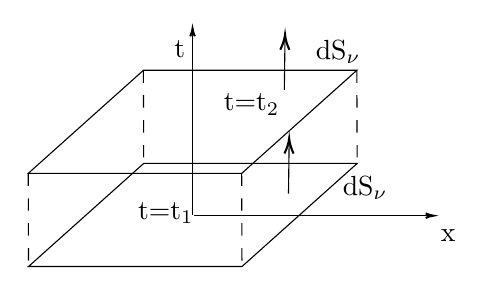
\begin{tikzpicture}[x=0.25pt,y=0.25pt,yscale=-1,xscale=1]
%uncomment if require: \path (0,514); %set diagram left start at 0, and has height of 514

%Straight Lines [id:da944915482116456] 
\draw    (250.32,299.23) -- (250.32,32) ;
\draw [shift={(250.32,30)}, rotate = 90] [color={rgb, 255:red, 0; green, 0; blue, 0 }  ][line width=0.75]    (10.93,-3.29) .. controls (6.95,-1.4) and (3.31,-0.3) .. (0,0) .. controls (3.31,0.3) and (6.95,1.4) .. (10.93,3.29)   ;
%Straight Lines [id:da15966795743012707] 
\draw    (252.32,300.23) -- (596.16,300.23) ;
\draw [shift={(598.16,300.23)}, rotate = 180] [color={rgb, 255:red, 0; green, 0; blue, 0 }  ][line width=0.75]    (10.93,-3.29) .. controls (6.95,-1.4) and (3.31,-0.3) .. (0,0) .. controls (3.31,0.3) and (6.95,1.4) .. (10.93,3.29)   ;
%Shape: Rectangle [id:dp13264483463125742] 
\draw   (179.7,224.73) -- (488.23,224.73) -- (321.76,373.73) -- (13.23,373.73) -- cycle ;
%Shape: Rectangle [id:dp5241947086840221] 
\draw   (179.29,90.11) -- (487.82,90.11) -- (321.35,239.11) -- (12.82,239.11) -- cycle ;
%Straight Lines [id:da9873328008653245] 
\draw    (383,118.5) -- (383.98,40.5) ;
\draw [shift={(384,38.5)}, rotate = 90.72] [color={rgb, 255:red, 0; green, 0; blue, 0 }  ][line width=0.75]    (21.86,-6.58) .. controls (13.9,-2.79) and (6.61,-0.6) .. (0,0) .. controls (6.61,0.6) and (13.9,2.79) .. (21.86,6.58)   ;
%Straight Lines [id:da7100914300813527] 
\draw    (389,268.5) -- (389.98,190.5) ;
\draw [shift={(390,188.5)}, rotate = 90.72] [color={rgb, 255:red, 0; green, 0; blue, 0 }  ][line width=0.75]    (21.86,-6.58) .. controls (13.9,-2.79) and (6.61,-0.6) .. (0,0) .. controls (6.61,0.6) and (13.9,2.79) .. (21.86,6.58)   ;
%Straight Lines [id:da5752286958121103] 
\draw  [dash pattern={on 4.5pt off 4.5pt}]  (12.82,239.11) -- (13.23,373.73) ;
%Straight Lines [id:da3625750970621462] 
\draw  [dash pattern={on 4.5pt off 4.5pt}]  (179.29,90.11) -- (179.7,224.73) ;
%Straight Lines [id:da36524075127919386] 
\draw  [dash pattern={on 4.5pt off 4.5pt}]  (487.82,90.11) -- (488.23,224.73) ;
%Straight Lines [id:da5000478553674463] 
\draw  [dash pattern={on 4.5pt off 4.5pt}]  (321.35,239.11) -- (321.76,373.73) ;

% Text Node
\draw (210,32.51) node [anchor=north west]   [align=left] {{t }};
% Text Node
\draw (595,306.78) node [anchor=north west]   [align=left] {{x}};
% Text Node
\draw (266,267) node [anchor= north east]   [align=left] {{ t=t\textsubscript{1}}};
% Text Node
\draw (268,110) node [anchor=north west]   [align=left] {{ t=t\textsubscript{2}}};
% Text Node
\draw (401,32) node [anchor=north west]   [align=left] {{ dS\textsubscript{$\nu $}}};
% Text Node
\draw (440,260) node [anchor=  west]   [align=left] {{ dS\textsubscript{$\nu $}}};
\end{tikzpicture}
\end{minipage}
\begin{minipage}[t]{0.48\textwidth}
    \vspace*{0pt} 
    This is an integral of the flux along the time direction. \par
    So the expression of $\Delta p^{\mu }_{ \text{ total }}$ can be written as \par
\end{minipage}

\[
= \int_{ \text{ total surface }}^{}{dS_{\nu }T^{\mu \nu }} = \int_{Volume}^{}{dx^{3}\partial_{\nu }T^{\mu \nu }} = \int_{volume}^{}{dV \partial_{\nu }T^{\mu \nu }}
\]
So we have two surfaces and we closed it inside a solid, and it is like we are doing gauss theorem, We can use the divergence theorem in 4d. We state that the divergence of $T^{\mu \nu }$:
\begin{gather*}
\partial_{\mu }T^{\mu \nu } = 0 \\
\partial_{\nu }T^{\mu \nu } = 0
\end{gather*}
And that's a way to express conservation.

\paragraph{Results for perfect fluids}
\[
T^{\mu \nu } = \left( \rho  +p \right) u^{\mu }u^{\nu }+p \eta^{\mu \nu }
\]
and taking the derivative
\begin{gather*}
\partial_{\mu } T^{\mu \nu } = \partial_{\mu }\left( \rho +p \right)u^{\mu }u^{\nu } + \partial_{\mu }p \eta^{\mu \nu } + \left( \rho +p \right)\left( \partial_{\mu }u^{\mu } \right)u^{\nu } + \left( \rho +p \right) u^{\mu }\partial_{\mu }u^{\nu } = \\
= \partial_{\mu }\left( \rho +p \right)u^{\mu }u^{\nu }+ \partial_{\mu }p \eta^{\mu \nu } + \left( \rho +p \right) [\left( \partial_{\mu }u^{\mu }u^{\nu } + u^{\mu }\partial_{\mu }u^{\nu } \right)]
\end{gather*}
It is quite clear, just the thing that we neglect derivative of the metric because in flat spacetime it is a constant matrix, and so it's 0.\par
Let's take the projection of this identity along the direction of the four-velocity.
\begin{gather*}
	u_{\nu }\partial_{\mu }T^{\mu \nu } = -\partial_{\mu }\left( \rho +p \right)u^{\mu }+\left( \partial_{\mu }p \right)u^{\mu }+\left( \rho +p \right)[-\partial_{\mu }u^{\mu }+u_{\nu }u^{\mu }\partial_{\mu }u^{\nu }] =
\end{gather*}
and since, 
\[
\partial_{\mu }\left( u_{\nu }u^{\nu } \right) = 0 = \partial_{\mu }\left( -1 \right)
\]
we get
\begin{equation}
= -\partial_{\mu }\left( \rho +p \right)u^{\mu } + \partial_{\mu }p u^{\mu }- \left( \rho +p \right)\partial_{\mu }u^{\mu } = 0
\end{equation}
And in the NR limit, $p\ll \rho $:
\begin{gather*}
-\partial_{\mu }\rho  u^{\mu }+\rho \partial_{\mu }u^{\mu }+ \partial_{\mu }pu^{\mu }=0 \\
\text{ we can neglect the last term since the hypothesis } \\
\partial_{\mu }\left( \rho u^{\mu } \right) = 0 \implies \partial_{t}\rho +\partial_{i}\left( \rho u^{i} \right) = 0
\end{gather*}
we recover the continuity equation.

\paragraph{exercise}: instead of projecting on $u^{\nu  }$, project orthogonal to $u^{\mu }$,compute: $p^{\alpha }_{\nu } \partial_{\mu }T^{\mu \nu }=0$.
idk what it means: $p^{\alpha }_{\beta }\equiv \delta^{\alpha }_{\beta } + u^{\alpha }u_{\beta }$. Evaluate alpha = 1,2,3.






\section{Lec 7}

\subsection{Equivalence Principle}

The idea of the \emph{universality} of the gravitational interaction, in the form of the \emph{Equivalence principle } led Einstein to think that gravity is special, not just another field, but a metric tensor that describes the curvature of spacetime.

\subsubsection{Weak Equivalence Principle, WEP}
It states that \emph{inertial} mass and \emph{gravitational} mass of any object are equal. \par
From the Second Law of Mechanics:
\[
 \vec{F}= m_{i}\vec{a}
\]
with $m_{i}=$ inertial mass.
While to quantify gravitational forces in Newtonian mechanics:
\[
\vec{F} = -m_{g} \nabla \Phi_{g}
\]
With $\nabla \Phi_{g}$ gradient of scalar field $\Phi_{g}$, known as gravitational potential.
From these formulas, we see no actual reason why $m_{i} = m_{g}$:
\begin{itemize}
	\item The inertial mass has a universal character, it takes the same value no matter what kind of force is being exerted.
	\item The gravitational mass is a quantity specific to the gravitational force. One could think $ \frac{m_{g}}{m_{i}}$ as the \emph{gravitational charge}.
\end{itemize}
Galileo showed by rolling balls down the inclined plane, that the response of matter to gravitation is universal, and in Newtonian mechanics it translates in WEP:
\[
m_{i }= m_{g}
\]
This, for freely falling objects, becomes
\[
a = -\nabla \Phi 
\]

This led to think an equivalent formulation of WEP that is: \emph{there exists a preferred class of trajectories through space time, called Inertial or Freely-Falling}.
Freely falling is intended as "moving under the sole influence of gravity", these objects are unaccelerated. \par

The universality of gravitation can be stated in another form:
\indent If we consider a physicist in a spaceship that is accelerating at a constant rate, like
\[
\vec{a} = - \vec{g}
\]
he would be not able to distinguish by scientific experiments the situation in which he sits on Earth's surface. (Restricted to local observation).


\tikzset{every picture/.style={line width=0.75pt}} %set default line width to 0.75pt

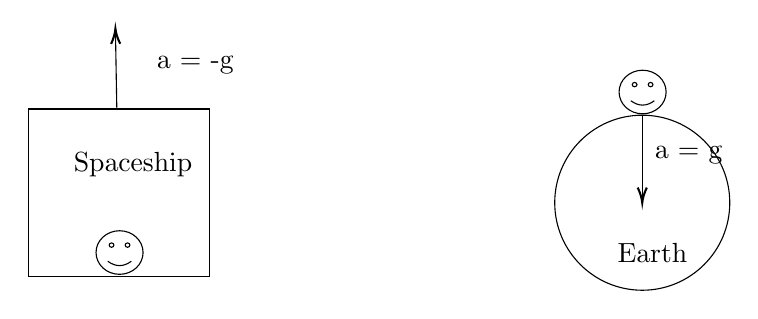
\begin{tikzpicture}[x=0.5pt,y=0.5pt,yscale=-1,xscale=1]
%uncomment if require: \path (0,300); %set diagram left start at 0, and has height of 300

%Shape: Rectangle [id:dp8176008658551641]
\draw   (98,85.5) -- (229,85.5) -- (229,206.5) -- (98,206.5) -- cycle ;
%Shape: Circle [id:dp5519338819044518]
\draw   (478.5,153.25) .. controls (478.5,118.32) and (506.82,90) .. (541.75,90) .. controls (576.68,90) and (605,118.32) .. (605,153.25) .. controls (605,188.18) and (576.68,216.5) .. (541.75,216.5) .. controls (506.82,216.5) and (478.5,188.18) .. (478.5,153.25) -- cycle ;
%Shape: Smiley Face [id:dp2317824195662611]
\draw   (147,189.25) .. controls (147,180.55) and (154.61,173.5) .. (164,173.5) .. controls (173.39,173.5) and (181,180.55) .. (181,189.25) .. controls (181,197.95) and (173.39,205) .. (164,205) .. controls (154.61,205) and (147,197.95) .. (147,189.25) -- cycle ; \draw   (156.52,183.9) .. controls (156.52,183.03) and (157.28,182.32) .. (158.22,182.32) .. controls (159.16,182.32) and (159.92,183.03) .. (159.92,183.9) .. controls (159.92,184.76) and (159.16,185.47) .. (158.22,185.47) .. controls (157.28,185.47) and (156.52,184.76) .. (156.52,183.9) -- cycle ; \draw   (168.08,183.9) .. controls (168.08,183.03) and (168.84,182.32) .. (169.78,182.32) .. controls (170.72,182.32) and (171.48,183.03) .. (171.48,183.9) .. controls (171.48,184.76) and (170.72,185.47) .. (169.78,185.47) .. controls (168.84,185.47) and (168.08,184.76) .. (168.08,183.9) -- cycle ; \draw   (155.5,195.55) .. controls (161.17,199.75) and (166.83,199.75) .. (172.5,195.55) ;
%Shape: Smiley Face [id:dp04372115955443423]
\draw   (525,73.25) .. controls (525,64.55) and (532.61,57.5) .. (542,57.5) .. controls (551.39,57.5) and (559,64.55) .. (559,73.25) .. controls (559,81.95) and (551.39,89) .. (542,89) .. controls (532.61,89) and (525,81.95) .. (525,73.25) -- cycle ; \draw   (534.52,67.9) .. controls (534.52,67.03) and (535.28,66.32) .. (536.22,66.32) .. controls (537.16,66.32) and (537.92,67.03) .. (537.92,67.9) .. controls (537.92,68.76) and (537.16,69.47) .. (536.22,69.47) .. controls (535.28,69.47) and (534.52,68.76) .. (534.52,67.9) -- cycle ; \draw   (546.08,67.9) .. controls (546.08,67.03) and (546.84,66.32) .. (547.78,66.32) .. controls (548.72,66.32) and (549.48,67.03) .. (549.48,67.9) .. controls (549.48,68.76) and (548.72,69.47) .. (547.78,69.47) .. controls (546.84,69.47) and (546.08,68.76) .. (546.08,67.9) -- cycle ; \draw   (533.5,79.55) .. controls (539.17,83.75) and (544.83,83.75) .. (550.5,79.55) ;
%Straight Lines [id:da28786648084951405]
\draw    (162,84.5) -- (161.04,29.5) ;
\draw [shift={(161,27.5)}, rotate = 88.99] [color={rgb, 255:red, 0; green, 0; blue, 0 }  ][line width=0.75]    (10.93,-3.29) .. controls (6.95,-1.4) and (3.31,-0.3) .. (0,0) .. controls (3.31,0.3) and (6.95,1.4) .. (10.93,3.29)   ;
%Straight Lines [id:da9125944015659164]
\draw    (541.75,90) -- (541.75,151.25) ;
\draw [shift={(541.75,153.25)}, rotate = 270] [color={rgb, 255:red, 0; green, 0; blue, 0 }  ][line width=0.75]    (10.93,-3.29) .. controls (6.95,-1.4) and (3.31,-0.3) .. (0,0) .. controls (3.31,0.3) and (6.95,1.4) .. (10.93,3.29)   ;

% Text Node
\draw (189,46) node [anchor=north west][inner sep=0.75pt]   [align=left] {a = -g};
% Text Node
\draw (549,111) node [anchor=north west][inner sep=0.75pt]   [align=left] {a = g};
% Text Node
\draw (522,181) node [anchor=north west][inner sep=0.75pt]   [align=left] {Earth};
% Text Node
\draw (129,115) node [anchor=north west][inner sep=0.75pt]   [align=left] {Spaceship};


\end{tikzpicture}
\bigskip\hfill

If the spaceship would be sufficiently big, we would see that the effect of acceleration would always be in the same direction, while on the surface or the Earth we would see that it points towards the center of the earth, so radial vs straight parallel lines.\par
So WEP could be stated as \emph{the motion of freely-falling particles are the same in a gravitational field and a uniformly accelerated frame, in small enough regions of spacetime}. In larger regions there would be inhomogenities, which will lead to tidal forces.

\subsubsection{Einstein's Equivalence Principle, EEP}
The Einstein Equivalence Principle is just a little generalization of the WEP:
\begin{quote}
In small enough regions of spacetime, the laws of physics reduce to those of special relativity: it is impossible to detect the existence of gravitational field by means of local experiments.
\end{quote}
Consider a hydrogen atom, a bound state of a proton and an electron. Its mass
is actually less than the sum of the masses of the proton and electron considered
individually, because there is a negative binding energy—you have to put energy
into the atom to separate the proton and electron. According to the WEP, the  gravitational mass of the hydrogen atom is therefore less than the sum of the masses of its constituents; the gravitational field couples to electromagnetism (which holds the atom together) in exactly the right way to make the gravitational mass come out right. This means that not only must gravity couple to rest mass universally, but also to all forms of energy and momentum—which is practically the claim of the EEP.

It is the EEP that implies that we should attribute the action of gravity the curvature of spacetime.

\subsubsection{Strong Equivalence Principle, SEP}
Is defined to include all of the laws of physics, gravitational and otherwise.
We will define \emph{unaccelerated} as \emph{freely falling}, from here we decide that gravity is not a force, because a force leads to acceleration, and our definition of zero acceleration is \emph{ moving freely in the presence of whatever gravitational field happens to be around.} \par

We know that there is a class of preferred frames: Inertial Frames (where laws of dynamics are true).
We introduce a new class of frames: Freely Falling Frames, where \emph{ unaccelerated particles move only due to gravity.} \par
Obviously these frames must be local frames, otherwise, due to inhomogenities on the gravitational field, particles initially at rest will begin to move with respect to such frame.
\begin{figure}[h]
\centering
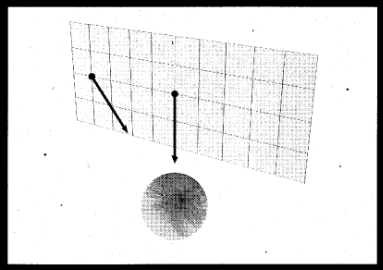
\includegraphics[width=0.8\linewidth]{imm/failureglobal.png}
\caption{The failure of global frames.}
\label{imm:failureglobal}
\end{figure}

After this we need a mathematical framework were what just said is consistent. The solution is to think that spacetime has a curved geometry and gravitation the manifestation of this curvature.
Before jumping in what is a manifold, let's see if the consequences are of our world.

\subsubsection{Gravitational Redshift}
\begin{figure}[h]
\centering
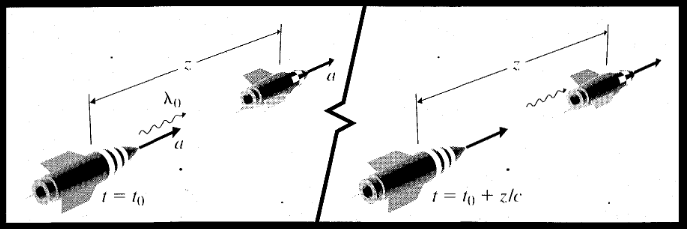
\includegraphics[width=0.8\linewidth]{imm/gravshift1.png}
\caption{Doppler shift measured by two rockets, each feeling acceleration \textbf{a}.}
\label{imm:gravshift1.png}
\end{figure}

Be two spaceships, separated by distance \emph{z}, each moving with constant $\vec{a}$ acceleration in a region without gravitational fields. \par
At \emph{t\textsubscript{0}} ship in the back emits a photos of $\lambda_{0}$.\par
The distance \emph{z} stays constant, so the photon is received after $\Delta t = z/c$ in our reference frame. At $t = t_{0}+ \Delta t$ the boxes have picked up an additional velocity $\Delta v = \vec{a}\Delta t = \vec{a}z/c$. The photon reaching the front spaceship will be redshifted bu the Doppler Effect, by \[
\frac{\Delta \lambda }{\lambda_{0}} = \frac{\Delta v}{c} = \frac{a z}{c^{2}}
\]
And according to EEP this should happen also in a uniform gravitational field.\par
\begin{figure}[h]
\centering
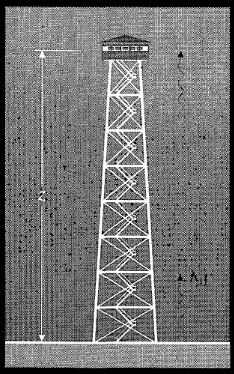
\includegraphics[width=0.3\linewidth]{imm/gravshift2.png}
\caption{Gravitational redshift on Earth's surface}
\label{imm:gravshift2}
\end{figure}
So i a photon e mitted from the ground with $\lambda_{0}$ will be redshifted by
\[
\frac{\Delta  \lambda }{\lambda_{0}} = \frac{a_{g}z}{c^{2}}
\]
To note that is a direct consequence of EEP, no details of GR were required.
The thing is, if i try to represent this with Minkowski metric, I don't notice the redshift.

So now we really need to talk about Manifolds
\subsection{Manifolds}
A manifold is a space that may be curved and have a complicated topology, but in local regions looks just like $\mathbb{R}^{n}$. A crucial part is that the dimensionality \emph{n} of the Euclidean Spaces being used must be the same in every patch of the manifold.
For example are not manifolds, a line ending on a plane and two cones intersecting at their vertices.\par
\begin{figure}[h]
\centering
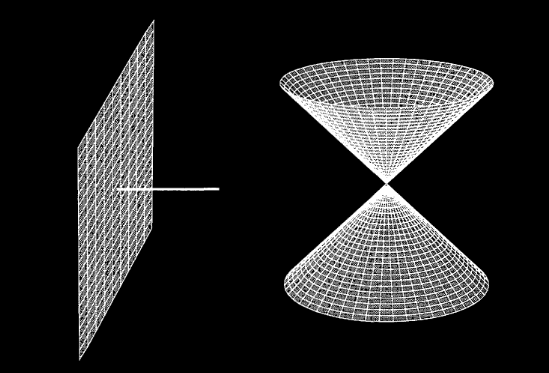
\includegraphics[width=0.5\linewidth]{imm/notmanifold.png}
\caption{Not manifolds}
\label{imm:notmanifold.png}
\end{figure}

\subsubsection{Coordinate System}
Be 
\begin{equation}
\begin{cases}
U\subset M \\
\phi : U \to \mathbb{R}^{n} \\
\phi\left( U \right) \text{ is open in }\mathbb{R}^{n}
\end{cases}
\end{equation}
These are a system of conditions to define a coordinate system or \emph{chart.}\par
\begin{figure}[h]
\centering
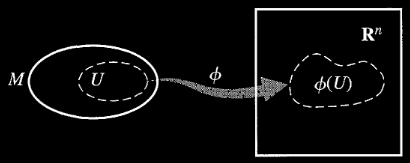
\includegraphics[width=0.65\linewidth]{imm/chart.png}
\caption{A coordinate chart covering an open subset \emph{U} of \emph{M}.}
\label{imm:chart}
\end{figure}
An \emph{atlas} is a indexed collection of charts $\{\left( U_{\alpha}, \phi_{\alpha } \right)\}$.

\subsubsection{Vectors again}
One point we stressed was the notion of a tangent space, the set of all vectors at a single point in spacetime. A vector is not a thing that stretches from one point to another but is an object associated with a single point. \par
Be $f : M \to \mathbb{R}$. Each curve passing through a point \emph{P}, defines an operator, the \emph{ directional derivative}, which maps $f \to df/d\lambda \left( \text{ at }p \right)$. \par
We claim the tangent space $T_{P}$ can be identified with the space of directional derivative operators along curves through \emph{P}.
And for any \emph{f} we can write:
\[
\frac{df}{d\lambda } = \frac{df}{dx^{\mu }} \frac{dx^{\mu }}{d\lambda } \implies \frac{d}{d\lambda } = \frac{dx^{\mu }}{d\lambda } \partial_{\mu }
\]
If i change the coordinates i can apply the chain rule.

\end{document}

